% !Mode:: "TeX:UTF-8"
\documentclass[review]{jcr}
%选项 preprint 提供手稿预览, 交叉引用颜色为蓝色
%    final    提交手稿时使用, 所有交叉引用颜色改为黑色
%    review   匿名评审模式, 打开之后编译时隐去作者信息
\usepackage[ruled]{algorithm2e}
\usepackage{hyperref}
\usepackage{amsmath}
\usepackage{amssymb}
\usepackage{color,xcolor}
\usepackage{graphicx,float}
\usepackage{framed}
\usepackage{lineno}
\usepackage{array}
\usepackage{graphicx}
\usepackage{multirow}
\usepackage{tikz}
\usepackage{pgfplots}
\usepackage{microtype} 
\usepackage{enumitem}


\setenumerate[1]{itemsep=0pt,partopsep=0pt,parsep=\parskip,topsep=1pt}
\setitemize[1]{itemsep=0pt,partopsep=0pt,parsep=\parskip,topsep=1pt}
\setdescription{itemsep=0pt,partopsep=0pt,parsep=\parskip,topsep=1pt}
\newtheorem{claim}{Claim}

\begin{document}
%% 编辑输入区 %%
\DOI{10.13868/j.cnki.jcr.0000XX}%文章DOI号
\vol{12}% 卷号
\issue{27}% 期号
\PrintDate{2017}{11}% 出版日期, 前者为年, 后者为月
\ReceivedDate{2016-05}% 收稿日期
\FinalVersionDate{2017-09}% 定稿日期
\PrintPage{1001}{1013}% 论文起止页码
\AuthorCiteInput{Tu B B, Chen Y}%输入英文引用格式中的英文作者姓名
%% 编辑输入区 %%

%% 以下内容均由作者提供 %%
\DocumentCode{A}%输入文献标识码
\CLCnumber{TP309.7}%输入中图分类号

\begin{frontmatter}
  % 输入中文标题
  % 输入中文标题
  \title{高效SM2适配器签名及其应用}

  % 输入英文标题
  \etitle{An Efficient SM2-based Adaptor Signature and Its Applications}

  % 输入基金项目
  \foundation{国家重点基础研究发展项目(973计划)(XXXXXXXXX); 国家自然科学基金项目(XXXXXXXX)}

  %------------- 输入作者信息 --------------%
    % 如果所有作者都在同一单位, 输入方法如下:
    % \author{作者一}% 输入作者中文姓名
    % \author{作者二}% \author 命令可以重复使用
    % \ead{Email}% 输入通讯作者的电子邮箱, 须紧随\author命令输入
    % \cortext{通讯作者}% 输入通讯作者, 此时通讯作者为上一个\author命令输入的作者, 并结合\ead命令显示通讯作者邮箱
    % \address{作者单位}% 输入作者单位

    % 如果多个作者在不同单位, 输入方法如下:
    % \author[biaoqian1,biaoqian2]{作者一}% 方括号内是引用自\address的标签
    % \address[biaoqian1]{作者一的第一单位} % 方括号内是标签, 由\author命令引用
    % \author[biaoqian2]{作者二}% 输入第二作者中文姓名
    % \ead{Email}% 输入通讯作者的电子邮箱, 须紧随\author命令输入
    % \cortext{通讯作者}% 输入通讯作者, 此时通讯作者为上一个\author命令输入的作者, 并结合\ead命令显示通讯作者邮箱
    % \address[biaoqian2]{作者一的第二单位}% 输入作者单位

    % 作者英文信息与上述方法相同
  %------------- 输入作者信息 --------------%

  % 输入作者中文及通讯作者信息
   \author[1]{涂彬彬}
   \author[1]{陈宇}
   \ead{E-mail: yuchen@sdu.edu.cn}
   \cortext{通讯作者}
  % \author[1,2]{作者二}
  % \author[1,2]{作者三}

  % % 输入作者英文及通讯作者信息
   \eauthor[1]{Tu Binbin}
   \eauthor[1]{Chen Yu}
   \ecortext{Corresponding author}
  % \eauthor[1,2]{ZUO Zhe-Er}
  % \eauthor[1,2]{ZUO Zhe-San}

  % % 输入作者附属单位中文
   \address[1]{山东大学 网络空间安全学院, 青岛\ 266237}
   
  % \address[2]{XXX研究院, 北京\ 100190}

  % % 输入作者附属单位英文
   \eaddress[1]{School of Cyber Science and Technology, Shandong University, Qingdao 266237, China}
  % \eaddress[2]{Academy of XXXX, Beijing 100190, China}

  \begin{abstract}
  适配器签名, 又名无脚本脚本, 是解决区块链应用 (如密码货币) 中扩展性差、 吞吐量低等问题的重要密码技术. 适配器签名可看作数字签名关于困难关系的扩展, 同时具有签名授权和证据提取两种功能, 在区块链应用中具有以下优点: (i) 降低链上成本, (ii) 提高交易的可替代性, (iii) 突破区块链脚本语言限制. SM2 签名是我国自主设计的国家标准算法, 在各种重要信息系统中有着广泛应用. 在本文中, 我们首次基于国密 SM2 签名构造了适配器签名方案, 并在随机预言机模型下基于SM2的安全性给出安全性证明. 随后, 我们根据 SM2 签名的结构特点, 采用离线证明技术进行优化, 获得了可支持离线证明的 SM2 适配器签名方案. 该方案与现有 ECDSA 适配器签名相比更加高效. 最后, 我们基于现有适配器签名应用, 分别给出 SM2 适配器签名在区块链中的两种典型应用: 原子交换协议和支付通道网络. 
  \end{abstract}

  % 输入中文关键词
  \begin{keywords}
    SM2算法; 适配器签名; 区块链; 原子交换; 支付通道网络
  \end{keywords}

  % 输入英文摘要
  \begin{eabstract}
   Adaptor signature, also known as scriptless scripts, is an important cryptographic technique that can be used to solve the problems of poor scalability and low transaction throughput in blockchain applications such as cryptocurrency. Adaptor signature can be seen as an extension of digital signature on hard relations, and it can tie together the authorization with witness extraction and has many advantages in blockchain applications, such as (i) low on-chain cost, (ii) improved fungibility of transactions, (iii) advanced functionality beyond the limitation of the blockchain's scripting language. SM2 signature is the Chinese national standard signature algorithm and has been widely used in various important information systems. In this paper, we first design the adaptor signature based on SM2 signature algorithm, and prove security based on SM2 security under the random oracle model. Then, based on the structure of SM2 signature, we use offline proof technique to optimize it and get a SM2-based adaptor signature supporting offline proof, which is more efficient than the existing ECDSA-based adapter signature. Finally, based on existing adapter signature applications, we show two applications of SM2-based adapter signature in blockchain: atomic swap protocol and payment channel network.

  \end{eabstract}

  % 输入英文关键词
  \begin{ekeywords}
    SM2; adaptor signature; blockchain; atomic swap; payment channel network
  \end{ekeywords}
\end{frontmatter}

\zihao{-5}

\section{引言}
自 2009 年比特币~\cite{Nak08}系统出现, 其底层的区块链结构引起了广泛关注. 区块链巧妙地融合了密码、共识机制、P2P 网络等关键技术, 具有去中心化、不可篡改、匿名性、可追溯性、开放透明等特点, 有着非常广阔的应用前景. 但相关区块链应用(如密码货币)也面临着可扩展性差、吞度量低等关键的应用问题~\cite{BanoSAAMMD19,GudgeonMRMG19,ZamyatinAZKMKK19,AumayrEEFHMMR20,SG2018}, 比如: 理论上, 比特币的交易吞吐量约为每秒十几笔, 与信用卡每秒数万笔的交易量相比, 低了三个数量级, 严重限制了区块链技术的广泛应用. 区块链上每笔交易可看作某种脚本构成的应用程序, 脚本语言定义了链上可实现的各种功能, 如比特币等支持签名授权的货币转账功能, 以太坊等提供图灵完备的脚本语言, 能够编码更复杂的交易逻辑实现更加丰富的应用功能. 然而, 愈加丰富的功能需要复杂的脚本支持, 导致链上的存储和矿工验证计算成本增加. 针对上述问题, 支付通道网络~\cite{PC2018}通过在链上建立通道, 可实现用户之间通过该通道进行任意次数的链下交易, 是目前最有前景和部署最广泛的解决方案之一, 如比特币的闪电网络~\cite{PD2016}和以太坊的雷电网络~\cite{raidEX}等. 适配器签名作为构建支付通道网络的关键技术, 是目前解决区块链可扩展性差, 减少链上资源等问题的重要工具. 

适配器签名(adaptor signature, AS) 由Poelstra~\cite{Poelstra2016}首次引入, 并由Aumayr等人~\cite{AumayrEEFHMMR20}给出形式化的定义. 适配器签名可看作是数字签名对困难关系(hard relation)的扩展. 简而言之, 签名者可以使用签名私钥对消息和困难实例进行预签名, 利用困难关系的证据可将预签名值转化为有效的完整签名值. 同时困难关系的证据可通过预签名值和完整签名值提取. 适配器签名具有以下特性: (i)只有拥有签名私钥的签名者才能生成预签名; (ii)只有拥有困难关系证据的用户才能将预签名值转化为完整签名值; (iii)获得预签名值和完整签名值, 可以验证两者的有效性, 并可提取困难关系的证据. 

在具体应用, 比如原子交换协议~\cite{Nolan2013,Poelstra2017,DeshpandeH20,Gugger20}中, 双方可基于适配器签名实现不同币种的公平交换. 一方 (困难关系选择方) 通过选择困难关系$(Y,y)$对交换交易进行预签名, 然后将预签名值$\hat{\sigma}_1$发送给另一方; 另一方根据困难实例$Y$也对交换交易进行预签名, 并将预签名值$\hat{\sigma}_2$返回;  困难关系选择方拥有困难关系的证据$y$可将预签名值$\hat{\sigma}_2$转换成交换交易的全签名值$\sigma_2$, 在链上公布签名值$\sigma_2$获得交换的货币; 另一方根据签名值$\sigma_2$和预签名值$\hat{\sigma}_2$可提取证据$y$, 并将预签名值$\hat{\sigma}_1$转换成交换交易的全签名值$\sigma_1$, 在链上公布签名值$\sigma_1$获得交换的货币. 至此, 双方完成公平交换交易. 根据上述应用的介绍, 适配器签名
通过将签名授权和证据提取巧妙地结合在一起完成货币交换的复杂操作, 具有减少链上操作, 提高交易的可替代性和突破区块链脚本语言限制等多种优势, 在许多区块链应用中都显示出了重要的应用价值, 如支付通道网络~\cite{DeckerW15,PC2018,AumayrEEFHMMR20}、支付通道网络中的支付路由~\cite{EckeyFHR20,MalavoltaMSKM19,MillerBBKM19}和原子交换协议~\cite{Nolan2013,Poelstra2017,DeshpandeH20,Gugger20}等. 


SM2签名算法~\cite{SM2,SM2-survey}是我国国家密码管理局公布的一种拥有完全自主知识产权的国家标准签名算法. 该算法基于椭圆曲线密码体制, 具有安全性高、签名速度快、占用空间小等优势, 在我国商密领域各类信息系统中有着重要应用. 现有的适配器签名主要基于Schnorr签名~\cite{Sch89,Poelstra2016,AumayrEEFHMMR20,ErwigFHMR2021}、ECDSA签名~\cite{ECDSA,rfc6605,AumayrEEFHMMR20,PA18}, 以及格签名~\cite{DucasLLSSS2018,EsginEE20}等方案构造, 缺少基于SM2算法的适配器签名方案, 限制了SM2算法在区块链场景下的推广应用. 此外, 现有基于ECDSA的适配器签名~\cite{AumayrEEFHMMR20} 在预签名值生成中需要零知识证明保证预签名的正确执行, 导致其预签名操作复杂, 应用效率较低. 秉承着核心技术自主创新、信息安全自主可控的理念, 本文主要探索基于SM2签名设计安全高效的SM2适配器签名方案, 为SM2算法在区块链场景中提供更加高效契合的应用参考, 为设计安全可控的区块链应用提供保障. 


\section{本文工作}  

在本文中, 我们首次基于国密SM2签名算法构造适配器签名方案, 并在随机预言机模型(random oracle model, ROM)下基于SM2签名的安全性给出适配器签名方案的可证明安全. 然后, 我们根据SM2签名的独特结构, 采用``离线证明技术''对SM2适配器签名进一步优化. 优化后的方案与现有ECDSA适配器签名方案(ECDSA-AS)~\cite{AumayrEEFHMMR20}相比, 在线预签名阶段的计算效率更高, 预签名尺寸更小. 随后, 我们对SM2适配器签名和ECDSA适配器签名进行理论和实验对比, 发现优化后的SM2适配器签名的在线预签名操作需要更少的点乘运算, 耗时仅为ECDSA适配器签名的1/4. 我们对相关技术介绍如下:

\begin{trivlist}
\item \textbf{SM2适配器签名.} SM2适配器签名是SM2签名和困难关系的扩展, 主要包含了预签名算法、预签名验证算法、适配算法、证据提取算法, 以及SM2的密钥生成算法、签名算法和签名验证算法. 其中, 预签名算法根据签名私钥和困难实例对消息进行预签名生成预签名值; 预签名验证算法可验证该预签名值的正确性; 适配算法可根据困难关系的证据将该预签名值转化为完整SM2签名值; 提取算法可根据预签名值和完整SM2签名值提取困难关系的证据. 具体而言, 令$(X,x)$为SM2签名算法的公私钥对, $(I=(Y,\pi),y)\in R_I$是离散对数困难关系~\cite{AumayrEEFHMMR20}. 签名方可计算预签名值: 计算点$Z=(x+1)Y$, 证明$X$和$Z-Y$具有相同的离散对数关系 ($Z-Y=xY, X=xG$): $\pi_Z\leftarrow \mathsf{P}((G,X,Y,Z-Y),x)$, 选择随机数$k$计算$\hat{K}=kG+Z=(k+y(x+1))G=\hat{k}G=(r_x,r_y)$, $r=r_x+h(m)$, $\hat{s}=(1+x)^{-1}(k-r\cdot x)$, 即预签名值$\hat{\sigma}=(r,\hat{s},Z,\pi_Z)$. 适配器算法可基于证据$y$将$\hat{\sigma}$转化为完整SM2签名值$\sigma=(r,s)$, 其中$s=\hat{s}+y=(x+1)^{-1}(k+y(x+1)-r\cdot x)=(x+1)^{-1}(\hat{k}-r\cdot x)$. 
\end{trivlist}

\begin{trivlist}
\item \textbf{可证明安全.} SM2适配器签名采用具有在线提取器性质的非交互零知识证明~\cite{Fischlin05}提供的``自证明结构''~\cite{AumayrEEFHMMR20}保证可证明安全. 具体而言, $(I=(Y,\pi),y)\in R_I$是具有``自证明结构''的离散对数困难关系~\cite{AumayrEEFHMMR20}, 其中$\pi\leftarrow \mathsf{P}(Y,y)$证明存在证据$y$使得$Y=y\cdot G$. 在安全性证明中, 根据困难关系的``自证明结构'',  归约算法在随机预言机模型下能提取证据$y$, 然后可基于SM2签名预言机输出的完整签名值$\sigma=(r,s)$, 并通过计算$\hat{s}=s-y$模拟SM2适配器签名的预签名预言机. 因此,如果存在敌手可伪造SM2适配器签名的预签名值$\hat{\sigma}^*=(r^*,\hat{s}^*)$,则归约算法可根据提取的证据$y$伪造SM2的签名值$\sigma^*=(r^*,s^*), 其中 s^*=\hat{s}^*+y$, 打破SM2签名的安全性, 从而证明SM2适配器签名的安全性基于SM2签名的安全性.
\end{trivlist}

\begin{trivlist}
\item \textbf{离线证明优化技术.} SM2适配器签名和现有ECDSA适配器签名~\cite{AumayrEEFHMMR20}都需要使用零知识证明保证预签名的正确执行. 不同的是,  SM2适配器签名的零知识证明与消息值及预签名使用的随机数无关. 因此, 零知识证明部分可以离线执行, 提升在线预签名操作的效率. 具体而言, 在预签名过程中, ECDSA-AS需要以预签名的随机数作为证据, 证明离散对数相等的困难关系$\{((G,K,Y,\hat{K}),k)|\exists\ k\in \mathbb{Z}_n,\ \text{s.t.}\ \hat{K}=kG\wedge K=kY\}$. 因此, 该证明只能由预签名方生成, 而且多次预签名计算需要选用不同的随机数, 对于新的随机数需要进行新的零知识证明. 

根据SM2签名的结构特点, 预签名过程可使用预签名私钥$x$作为证据, 证明离散对数相等的困难关系$\{((G,X,Y,Z),x)|\exists\ x\in \mathbb{Z}_n,\ \text{s.t.}\ X=xG\wedge Z-Y=xY\}$. 同时根据$Z=(x+1)Y=y(X+G)$的结构, 也能使用$y$为证据, 证明离散对数相等的困难关系$\{((G,Y,X+G,Z),y)|\exists\ y\in \mathbb{Z}_n,\ \text{s.t.}\ Z=y(X+G)\wedge Y=yG\}$. 根据$Z$结构的两种证明方式, 可对应SM2适配器签名更丰富且灵活的应用:(i) 以预签名私钥$x$为证据时, 关于$Z$结构的证明只能由预签名方生成(类似ECDSA-AS);(ii)以$y$为证据时, 关于$Z$结构的证明可由困难关系选择方生成.
因此, 我们可采用``离线证明技术''对SM2适配器签名进行优化, 设计更加高效的SM2适配器签名方案. 令SM2-ASv1表示SM2适配器签名方案, SM2-ASv2表示优化后的SM2适配器签名方案. SM2-ASv2采用离线证明技术并不影响其``自证明结构'', 可保证在安全性证明中归约算法提取证据$y$. 因此, 上述优化提升SM2适配器签名预签名阶段的效率, 不影响SM2-ASv2的安全性.
\end{trivlist}

\begin{trivlist}
\item \textbf{性能评估.} 我们分别通过理论和实验分析, 对现有ECDSA-AS~\cite{PA18,AumayrEEFHMMR20}, SM2-ASv1/2进行对比. 在线预签名阶段, ECDSA-AS需要证明离散对数相等关系, 
而根据SM2签名算法特性, SM2-ASv2可进行离线证明, 因此适配器签名SM2-ASv2比ECDSA-AS~\cite{PA18,AumayrEEFHMMR20}更加高效. 随后, 基于OpenSSL, 我们实现了ECDSA-AS~\cite{AumayrEEFHMMR20}, SM2-ASv1/2, 对比了三种方案的在线预签名算法和预签名验证算法的计算效率.  实验结果显示SM2-ASv2的在线预签名耗时仅为ECDSA-AS~\cite{AumayrEEFHMMR20}的1/4, 实验结果符合具体理论分析.
\end{trivlist}

\begin{trivlist}
\item \textbf{应用推广.} 
在现有适配器签名应用基础上~\cite{Poelstra2017,MalavoltaMSKM19,EsginEE20,AumayrEEFHMMR20}, 我们分别给出SM2适配器签名在区块链中的两种典型应用: 原子交换协议~\cite{Nolan2013,Poelstra2017,DeshpandeH20,Gugger20}和支付通道网络~\cite{DeckerW15,PC2018,AumayrEEFHMMR20}, 分别实现跨链货币公平交换功能和支付通道网络下多跳支付功能, 为SM2适配器签名的具体应用推广提供参考. 
\end{trivlist}

\section{预备知识} 

\subsection{符号}

本文中, 用 $\mathbb{N}$ 表示自然数集, 用 $\lambda\in \mathbb{N}$ 表示安全参数. 对任意 $n \in \mathbb{N}$, 符号 $[1,n]$ 表示集合 $\{1,\cdots,n\}$. 对任意有限集 $X$, $x \leftarrow X$ 表示从 $X$ 中均匀随机地选取出一个元素 $x$. 

关于安全参数 $\lambda$ 的函数$\mathsf{negl}$, 如果 $\mathsf{negl}(\lambda) \geq 0$, 而且对任意正多项式 $\mathsf{poly}$, 存在正整数 $c \in \mathbb{N}$, 使得对于所有的 $n \geq c$ 满足 $\mathsf{negl}(n) \leq \frac{1}{\mathsf{poly}(n)}$, 我们称函数$\mathsf{negl}$是可忽略的.   
对任意概率算法 $\mathcal{A}$, 记 $\mathcal{A}$ 所用的随机数集合为 $R$. $y \leftarrow \mathcal{A}(x_1,\cdots,x_t;r)$ 表示 $\mathcal{A}$ 以 $(x_1, \cdots, x_t)$ 和随机数 $r\leftarrow R$为输入, 输出 $y$; 通常我们忽略$r$, 记为 $y \leftarrow \mathcal{A}(x_1,\cdots,x_t)$. 如果 $\mathcal{A}$ 的运行时间是关于安全参数 $\lambda$ 的多项式, 则称 $\mathcal{A}$ 为概率多项式时间(probabilistic polynomial time, PPT)算法. 


\subsection{签名}
签名方案~\cite{AumayrEEFHMMR20}包含三个多项式时间算法$\sum=(\mathsf{Gen},\mathsf{Sign},\mathsf{Vrfy})$, 具体定义如下: 

\begin{itemize}
\item $\mathsf{Gen}(1^\lambda)$: 密钥生成算法输入安全参数$\lambda$, 输出签名密钥对$(vk,sk)$. 
\item $\mathsf{Sign}(sk,m)$: 签名算法输入签名私钥$sk$和消息$m\in\{0,1\}^*$, 输出签名值$\sigma$. 
\item $\mathsf{Vrfy}(vk,m,\sigma)$: 验证算法输入验证公钥$vk$, 消息$m\in\{0,1\}^*$和签名值$\sigma$, 输出$1$代表签名正确, 否则输出$0$. 
\end{itemize}

\begin{trivlist}
\item \textbf{正确性.}对任意$\lambda\in \mathbb{N}$, $(vk,sk)\leftarrow \mathsf{Gen}(1^\lambda)$, $m\in\{0,1\}^*$, 则$\Pr[\mathsf{Vrfy}(vk,m,\mathsf{Sign}(sk,m))\rightarrow 1]=1$. 
\end{trivlist}
\begin{trivlist}
\item \textbf{SUF-CMA 安全.}如果对于任意PPT敌手$\mathcal{A}$, 存在可忽略函数$\mathsf{negl}$, 使得在实验$\text{sSigForge}_{\sum,\mathcal{A}}$中, 敌手优势
$\textbf{Adv}_{\mathcal{A},\text{sSigForge}}=$$\Pr[\text{sSigForge}_{\sum,\mathcal{A}}(\lambda)=1]\leq \mathsf{negl}(\lambda)$, 则称签名方案$\sum$是选择消息攻击下强不可伪造(strong existential unforgeablity under chosen message attack, SUF-CMA), 其中实验 $\text{sSigForge}_{\sum,\mathcal{A}}$ 定义如下: 

\begin{center}
\fbox{
\begin{tabular}{lll}
 $\text{sSigForge}_{\mathcal{A},\sum}(\lambda)$ & \ \  & $\mathcal{O}_{\text{S}}(m)$ \\
\cline{1-1} \cline{3-3}

  $\mathcal{Q}=\emptyset$& \ \  & $\sigma\leftarrow \mathsf{Sign}(sk,m)$ \\
  $(vk,sk)\leftarrow \mathsf{Gen}(1^\lambda)$& \ \  & $\mathcal{Q}=\mathcal{Q}\cup \{m,\sigma\}$ \\
  $(m,\sigma)\leftarrow \mathcal{A}^{\mathcal{O}_{\text{S}}(\cdot)}(vk)$& \ \  & \textbf{return} $\sigma$ \\
  \textbf{return} $((m,\sigma)\notin \mathcal{Q}\wedge \mathsf{Vrfy}(vk,m,\sigma))$& \ \  &  \\

\end{tabular}}
\end{center}

\end{trivlist}


\subsection{SM2签名}
令$\mathbb{G}$为椭圆曲线上的群, $G$为群$\mathbb{G}$中阶为$n$的基点. 随机选择签名私钥$x\in [1,n-2]$, 计算验证公钥$X=xG$. 为了方便, 本文省略SM2的编码部分, 具体可见SM2签名标准~\cite{SM2}. 

关于消息$m \in \{0, 1\}^*$的SM2签名步骤如下: 

\begin{itemize}
\item[1.] 计算$e = H(m)$\footnote{其中$H(\cdot)$表示哈希函数, 具体可见SM2签名标准~\cite{SM2}}. 
\item[2.] 选择随机数$k\in [1,n-1]$, 计算$r_x=f(kG)$\footnote{SM2的变换函数$f$与ECDSA类似, 被定义为点$kG$的横坐标, 即$kG=(r_x,r_y)$, $r_x=f(kG)$~\cite{ZhangYZC15,AumayrEEFHMMR20}.}. 
\item[3.] 计算$r = r_x + e \bmod n$, 如果$r = 0$ 或者 $r + k = n$则返回步骤2. 
\item[4.] 计算 $s=(1+x)^{-1}(k-rx) \bmod n$, 如果$s=0$则返回步骤2. 
\item[5.] 输出签名值$\sigma = (r, s)$. 
\end{itemize}

SM2签名$\sigma = (r, s)$的验证步骤如下:  
\begin{itemize}
\item[1.] 如果$r\notin [1,n − 1]$ 或者 $s\notin [1,n − 1]$, 输出$0$并退出.
\item[2.] 计算$e = H(m)$. 
\item[3.] 计算$t=(r+s) \bmod n$, 如果$t=0$, 输出$0$并退出. 
\item[4.] 计算$r_x'=f(sG+tX)$. 
\item[5.] 计算 $r'=r_x'+e \bmod n$, 如果$r'=r$则输出$1$否则输出$0$. 
\end{itemize}

SM2签名算法是我国自主研发的签名算法, 具有安全性高, 运算速度快, 签名尺寸小等优势. SM2签名算法的安全性分析已有较多工作, 具体可参考~\cite{ZhangYZC15,SM2-survey,SM2}.

\subsection{困难关系和零知识证明}

令实例/证据对$(Y,y)$是一对关系, 定义语言$L_R=\{Y|\exists\ y, \text{s.t.} (Y,y)\in R\}$. $R$是困难关系~\cite{AumayrEEFHMMR20}, 如果以下条件成立: 
\begin{itemize}
  \item $\mathsf{GenR}(1^\lambda)\rightarrow (Y,y)$: 存在PPT取样算法$\mathsf{GenR}$输入$1^\lambda$, 输出关系$R$上的实例/证据对$(Y,y)\in R$.

  \item 该关系是多项式时间可判定的. 

  \item 对任意PPT\ 敌手$\mathcal{A}$, 输入困难实例$Y$输出证据$y$的概率是可忽略的.
\end{itemize}

对于困难关系$R$, 一组算法$(\mathsf{P},\mathsf{V})$是在随机预言机$\mathcal{H}$下具有在线提取器性质的非交互零知识的知识证明(non-interactive zero-knowledge proof of knowledge, NIZK-PoK)~\cite{AumayrEEFHMMR20,Fischlin05}, 需要满足以下条件: 

\begin{itemize}
  \item 完备性: 对于任意困难关系$(Y,y)\in R$, $\pi\leftarrow \mathsf{P}^{\mathcal{H}}(Y,y)$, 存在可忽略函数$\mathsf{negl}$, 使得$\Pr[$$\mathsf{V}^{\mathcal{H}}$$(Y$, $\pi)$$=1]$$\geq$ $1-\mathsf{negl}(\lambda)$. 
  \item 零知识性: 对于任意困难关系$(Y,y)\in R$, 存在PPT的模拟器$\mathcal{S}$输入实例$Y$可模拟证明$\pi$.
  \item 在线提取器: 存在PPT提取算法$\mathsf{K}$, 输入实例和证明$(Y,\pi)$ 可访问随机预言机的询问序列以及对应回复, 能提取证据$y$, 满足$(Y,y)\in R$.  
\end{itemize}

\subsection{适配器签名}
关于困难关系$R=(Y,y)$和签名$\sum=(\mathsf{Gen}$,$\mathsf{Sign}$,$\mathsf{Vrfy})$的适配器签名$\sum_{AS}=($$\mathsf{pSign}$, $\mathsf{pVrfy}$, $\mathsf{Adapt}$, $\mathsf{Ext})$~\cite{AumayrEEFHMMR20}, 定义如下: 

\begin{itemize}
  \item $\mathsf{pSign}(pk,sk,m,Y)\rightarrow \hat{\sigma}$. 预签名算法输入公钥$pk$、签名私钥$sk$、消息$m\in\{0,1\}^*$, 以及实例$Y$, 输出预签名值$\hat{\sigma}$.

  \item $\mathsf{pVrfy}(pk,m,Y,\hat{\sigma})\rightarrow 0/1$. 预签名验证算法输入公钥$pk$、消息$m\in\{0,1\}^*$、实例$Y$, 以及预签名值$\hat{\sigma}$, 如果预签名值验证成功输出$1$, 否则输出$0$.

  \item $\mathsf{Adapt}(\hat{\sigma},y)\rightarrow \sigma$.
  适配算法输入预签名值$\hat{\sigma}$和证据$y$, 输出签名值$\sigma$.

  \item $\mathsf{Ext}(\sigma,\hat{\sigma},Y)\rightarrow y$.
  提取算法输入签名值$\sigma$, 预签名值$\hat{\sigma}$和实例$Y$, 输出证据$y$.
\end{itemize}

适配器签名需要满足原签名的正确性, 还需要满足预签名的正确性, 以及预签名的可适配性. 简单来说, 预签名的正确性可保证签名方诚实地生成关于实例$Y\in L_R$的预签名值. 该预签名值能通过验证, 并且能被适配成一个有效的签名值. 基于该预签名值和适配后的完整签名值能提取出实例$Y$的证据. 该性质保证实例$Y\in L_R$的预签名能被适配成一个有效的签名值, 当且仅当签名方知道实例$Y$的证据$y$. 预签名的可适配性保证任意有效的预签名值和实例$Y$的证据$y$可以适配成一个有效的签名值, 即使该实例$Y$、预签名值由预签名方恶意地生成. 因此, 预签名的可适配性比预签名的正确性更强. 

\begin{trivlist}
\item \textbf{预签名正确性.}如果对任意的$\lambda\in \mathbb{N}$, $m\in\{0,1\}^*$, $(Y,y)\in R$有以下式子成立, 则称适配器签名满足预签名正确性.

\begin{equation*}
\begin{aligned}
\Pr\left[
\begin{array}{c|c}
\mathsf{pVrfy}(pk,\hat{\sigma},Y,m)= 1 & \mathsf{Gen}(1^\lambda)\rightarrow (sk,pk)\\
\wedge & \mathsf{pSign}((pk,sk),Y,m)\rightarrow \hat{\sigma} \\               
\mathsf{Vrfy}(pk,\sigma,m)= 1  & \mathsf{Adapt}(\hat{\sigma},y)\rightarrow \sigma \\
\wedge  & \mathsf{Ext}(\sigma,\hat{\sigma},Y)\rightarrow y' \\
(Y,y')\in R & \\
\end{array}
\right]=1
\end{aligned}
\end{equation*}

\end{trivlist}

\begin{trivlist}
\item \textbf{预签名可适配性.}如果对任意的$\lambda\in \mathbb{N}$, $m\in\{0,1\}^*$, $(Y,y)\in R$, $(pk,sk)\leftarrow \mathsf{Gen}(1^\lambda)$, 以及任意可验证成功的预签名$\hat{\sigma}$, $\mathsf{pVrfy}(pk,m,Y,\hat{\sigma})\rightarrow 1$, 都有 $\Pr[\mathsf{Vrfy}(pk$, $m$, $\mathsf{Adapt}(\hat{\sigma}$, $y))\rightarrow 1] = 1$, 则称适配器签名满足预签名可适配性. 
\end{trivlist}

适配器签名需要满足原签名方案的选择消息攻击下的存在不可伪造性(existential unforgeablity under chosen message attack, EUF–CMA), 还需要满足选择消息攻击下适配器签名的存在不可伪造性(EUF–CMA for adaptor signature, aEUF–CMA), 以及适配器签名的证据可提取性(witness extractability for adaptor signature, aWE). 具体安全性定义描述如下:

\begin{trivlist}
\item \textbf{选择消息攻击下适配器签名的存在不可伪造性.}对于任意的PPT敌手$\mathcal{A}$, 如果存在可忽略函数$\mathsf{negl}$, 使得敌手优势$\textbf{Adv}_{\mathcal{A},\text{aSigForge}}=$$\Pr[\text{aSigForge}_{\mathcal{A},\Pi_{R,\sum}}(\lambda) = 1] \leq \mathsf{negl}(\lambda)$成立, 则称适配器签名满足
aEUF–CMA, 其中$\text{aSigForge}_{\mathcal{A},\Pi_{R,\sum}}$定义如下: 
\end{trivlist}

\begin{center}
\fbox{
\begin{tabular}{lll}
 $\text{aSigForge}_{\mathcal{A},\Pi_{R,\sum}}(\lambda)$ & \ \  & $\mathcal{O}_{\text{S}}(m)$ \\
\cline{1-1} \cline{3-3}

 $\mathcal{Q}=\emptyset$ & \ \  & $\sigma\leftarrow \mathsf{Sign}(sk,m)$ \\

 $(pk,sk)\leftarrow \mathsf{Gen}(1^\lambda)$ & \ \  & $\mathcal{Q}=\mathcal{Q}\cup \{m\}$ \\

 $m\leftarrow \mathcal{A}^{\mathcal{O}_{\text{S}}(\cdot),\mathcal{O}_{\text{pS}}(\cdot)}(pk)$ & \ \  & return $\sigma$ \\
 $(Y,y)\leftarrow \mathsf{GenR}(1^\lambda)$ & \ \  &  \\
  $\hat{\sigma}\leftarrow \mathsf{pSign}((pk,sk),Y,m)$ & \ \  & $\mathcal{O}_{\text{pS}}(m,Y)$ \\
 \cline{3-3}

 $\sigma\leftarrow \mathcal{A}^{\mathcal{O}_{\text{S}}(\cdot),\mathcal{O}_{\text{pS}}(\cdot)}(\hat{\sigma},Y)$ & \ \  & $\hat{\sigma}\leftarrow \mathsf{pSign}((pk,sk),m,Y)$ \\

 return $(m\notin \mathcal{Q} \wedge \mathsf{Vrfy}(pk,m,\sigma))$ & \ \  & $\mathcal{Q}=\mathcal{Q}\cup \{m\}$  \\

  & \ \  & return $\hat{\sigma}$  \\
\end{tabular}}
\end{center}

除了提供额外的预签名预言机$\mathcal{O}_{\text{pS}}(\cdot)$, 适配器签名的 aEUF–CMA安全类似 EUF–CMA. 该预言机输入消息值和实例$Y$输出一个预签名值. 预签名预言机是非常关键的, 因为在应用中适配器签名要求敌手在不知道实例$Y$的证据的情况下, 即使知道预签名值也难以伪造消息的真实签名值. aEUF–CMA和预签名的可适配性一起保证了关于实例$Y$的预签名值能被转换成一个有效的签名值, 当且仅当知道实例$Y$的证据$y$. 

\begin{trivlist}
\item \textbf{证据可提取性.}对于任意的PPT敌手$\mathcal{A}$, 如果存在可忽略函数$\mathsf{negl}$, 使得在实验$\text{aWitExt}_{\mathcal{A},\Pi_{R,\sum}}$中敌手优势$\textbf{Adv}_{\mathcal{A},\text{aWitExt}}$$=$$\Pr[$$\text{aWitExt}_{\mathcal{A},\Pi_{R,\sum}}(\lambda) = 1] \leq \mathsf{negl}(\lambda)$, 则称适配器签名满足证据可提取性. $\text{aWitExt}_{\mathcal{A},\Pi_{R,\sum}}$定义如下: 
\end{trivlist}

\begin{center}
\fbox{
\begin{tabular}{lll}
 $\text{aWitExt}_{\mathcal{A},\Pi_{R,\sum}}(\lambda)$ & \ \  & $\mathcal{O}_{\text{S}}(m)$ \\
\cline{1-1} \cline{3-3}

 $\mathcal{Q}=\emptyset$ & \ \  & $\sigma\leftarrow \mathsf{Sign}(sk,m)$ \\

 $(pk,sk)\leftarrow \mathsf{Gen}(1^\lambda)$ & \ \  & $\mathcal{Q}=\mathcal{Q}\cup \{m\}$ \\

 $(m,Y)\leftarrow \mathcal{A}^{\mathcal{O}_{\text{S}}(\cdot),\mathcal{O}_{\text{pS}}(\cdot)}(pk)$ & \ \  & return $\sigma$ \\
 $\hat{\sigma}\leftarrow \mathsf{pSign}((pk,sk),Y,m)$ & \ \  &  \\
 $\sigma \leftarrow \mathcal{A}^{\mathcal{O}_{\text{S}}(\cdot),\mathcal{O}_{\text{pS}}(\cdot)}(\hat{\sigma})$  & \ \  & $\mathcal{O}_{\text{pS}}(m,Y)$ \\
 \cline{3-3}

 $y'\leftarrow \mathsf{Ext}(\sigma,\hat{\sigma},Y)$ & \ \  & $\hat{\sigma}\leftarrow \mathsf{pSign}((pk,sk),m,Y)$ \\

 return $(m\notin \mathcal{Q} \wedge (Y,y')\notin R$ & \ \  & $\mathcal{Q}=\mathcal{Q}\cup \{m\}$  \\

 $\wedge \mathsf{Vrfy}(pk,m,\sigma)$ & \ \  & return $\hat{\sigma}$  \\

\end{tabular}}
\end{center}

适配器签名的证据可提取性可保证关于消息和实例$(m,Y)$的一对有效的签名值和预签名值$(\sigma,\hat{\sigma})$ 能被用于提取出$Y$的证据$y$. 实验aWitExt和实验aSigForge的重要区别: 在实验aWitExt中, 敌手可选择实例$Y$. 因此, 在实验aWitExt中可认为敌手知道实例$Y$的证据$y$, 可以生成关于挑战消息$m$的有效签名值. 但是这个优势不足于让敌手赢得实验aWitExt, 因为敌手赢得实验aWitExt的条件是他输出的有效签名值不能泄漏实例$Y$的证据$y$. 

\begin{definition}
如果适配器签名$\sum_{AS}$满足预签名可适配性, aEUF–CMA安全和证据可提取性, 则称该适配器签名$\sum_{AS}$是安全的.
\end{definition}


\section{基于SM2的适配器签名} 

\subsection{方案设计}

本节中, 我们给出基于SM2的适配器签名方案, 并在随机预言机模型下给出安全性证明. 令$R=$ $\{$$(I_Y=(Y$, $\pi_Y)$, $y)$ $| Y = yG$ $\wedge$ $\mathsf{V}(Y, \pi_Y)$ $\rightarrow 1\}$, $R_Z= \{(I_Z=(G,X,Y,Z),x) | X = xG \wedge Z-Y=xY\}$, $\mathsf{P}$和$\mathsf{V}$分别表示零知识证明系统中的证明和验证算法. 基于SM2的适配器签名算法构造如下: 

\begin{itemize}

\item $\mathsf{pSign}((X,x),m,I_Y)\rightarrow \hat{\sigma}$. 预签名算法输入公私钥对 $(X,x)$, 消息值 $m$ 和困难实例 $I_Y=(Y, \pi_Y)$, 计算 $Z=(x+1)Y$, 运行 $\mathsf{P}(I_Z=(G,X,Y,Z),x)\rightarrow \pi_Z$, 计算 $e=H(m)$, 选择随机数$k\leftarrow \mathbb{Z}_n$, 并计算 $\hat{K}=kG+Z$, $r_x=f(\hat{K})$, $r=e+r_x$, $\hat{s}=(1+x)^{-1}(k-rx) \bmod n$, 最后输出预签名值$\hat{\sigma}=(r,\hat{s}, Z, \pi_Z)$.

\item $\mathsf{pVrfy}(X,m,I_Y,\hat{\sigma})\rightarrow 0/1$. 预签名验证算法输入公钥 $X$, 消息$m$, 困难实例$I_Y=(Y, \pi_Y)$, 以及预签名值 $\hat{\sigma}=(r,\hat{s}, Z, \pi_Z)$,  运行$\mathsf{V}(I_Z,\pi_Z)\rightarrow 0$, 则输出 $0$, 否则计算$e=H(m)$, $\hat{K}=(\hat{s}+r)X+\hat{s}G+Z$, $r'=f(\hat{K})+e \bmod n$. 如果 $r'=r$, 该算法输出 $1$, 否则输出 $0$. 

\item $\mathsf{Adapt}(\hat{\sigma},y)\rightarrow \sigma$. 适配算法输入预签名值$\hat{\sigma}$和证据$y$, 计算$s=\hat{s}+y \bmod n$, 并输出签名值$\sigma=(r,s)$. 

\item $\mathsf{Ext}(\sigma,\hat{\sigma},I_Y)\rightarrow y$. 证据提取算法输入签名值$\sigma$, 预签名值$\hat{\sigma}$和困难实例$I_{Y}=(Y, \pi_Y)$, 计算$y=s-\hat{s} \bmod n$. 如果$(Y, y)\in R$, 输出$y$, 否则输出 $\bot$. 
\end{itemize}
\ 
\begin{figure}
\begin{center}
\fbox{
\begin{tabular}{lllll}
$\mathsf{pSign}((X,x),m,I_Y)$ & \ \    & $\mathsf{pVrfy}(X,m,I_Y,\hat{\sigma})$ & \ \   & $\mathsf{Adapt}(\hat{\sigma},y)$ \\
\cline{1-1} \cline{3-3} \cline{5-5}

$pk=X,sk=x$& \ \  & $pk=X, I_Y=(Y,\pi_Y)$ & \ \  & $\hat{\sigma}=(r,\hat{s},Z,\pi_Z)$  \\

$I_Y=(Y,\pi_Y)$& \ \  & $\hat{\sigma}=(r,\hat{s},Z,\pi_Z)$ & \ \  &  $s=\hat{s}+y \bmod n$ \\

$Z=(x+1)Y$& \ \  & $b_Z\leftarrow \mathsf{V}(I_Z,\pi_Z)$& \ \   &  return $\sigma=(r,s)$ \\

$\mathsf{P}(I_Z,x)\rightarrow \pi_Z$& \ \  & $e=H(m)$ & \ \   &  \\

$e=H(m)$& \ \   & $\hat{K}=(\hat{s}+r)X+\hat{s}G+Z$ & \ \   & $\mathsf{Ext}(\sigma,\hat{\sigma},I_Y)$  \\
\cline{5-5}

$k\leftarrow \mathbb{Z}_n$& \ \  & $r'=f(\hat{K})+e \bmod n$& \ \   &  $\sigma=(r,s)$ \\

$\hat{K}=kG+Z,r_x=f(\hat{K})$& \ \  & $b_r=(r'=r)$& \ \   &  $\hat{\sigma}=(r,\hat{s},Z,\pi_Z)$ \\

$r=e+r_x$& \ \  & return $(b_Z \wedge b_r)$& \ \   & $I_Y=(Y,\pi_Y)$ \\

$\hat{s}=(1+x)^{-1}(k-rx) \bmod n$& \ \  & & \ \  &  $y=s-\hat{s} \bmod n$ \\

return $\hat{\sigma}=(r,\hat{s},Z,\pi_Z)$& \ \  &  & \ \   & If $(Y, y)\in R$, return $y$, \\

& \ \  &  & \ \  &  else return $\bot$  \\

\end{tabular}}
\caption{基于SM2的适配器签名}{SM2-based adaptor signature scheme}
\label{SM2-based adaptor signature scheme}
\end{center}
\end{figure}

\subsection{安全性证明}

\begin{theorem}
如果SM2签名$\sum_{\text{SM2}}$满足SUF–CMA, 且$R$是一个困难关系, 则上述方案$\Pi_{R,\sum_{\text{SM2}}}$在随机预言机模型下是安全的. 
\end{theorem}

\begin{lemma}(\emph{预签名的正确性.}) 基于SM2的适配器签名$\Pi_{R,\sum_{\text{SM2}}}$满足预签名的正确性. 
\end{lemma}

\begin{proof}
选定$x,y\in \mathbb{Z}_n$和$m\in \{0,1\}^*$, 定义$X=xG, Y=yG$, $\pi_Y\leftarrow \mathsf{P}((G,Y), y)$和$I_Y=(Y, \pi_Y)$. 根据预签名算法的定义$\mathsf{pSign}((X,x),m,I_Y)\rightarrow (r,\hat{s},Z,\pi_Z)$, 对于随机数$k\leftarrow \mathbb{Z}_n$,  $\hat{s}=(1+x)^{-1}(k-rx) \bmod n$.  令 $K=(\hat{s}+r)X+\hat{s}G=kG$. 

根据NIZK$_Z$的正确性, 即$\mathsf{V}(I_Z, \pi_Z)\rightarrow 1$. 因此, $Z=(x+1)Y=(x+1)yG$, $\hat{K}=K+Z=(k+y(x+1))G, r_x'=f(\hat{K}), r'=r_x'+e=r$, 即 $\mathsf{pVrfy}(X,m,I_Y,\hat{\sigma})\rightarrow 1$. 由于$\mathsf{Adapt}(\hat{\sigma}, y)\rightarrow \sigma$, 根据SM2签名的正确性 $\mathsf{Vrfy}(pk,m,\sigma)\rightarrow 1$. 因为 $\mathsf{Adapt}(\hat{\sigma}, y)\rightarrow \sigma$, 所以根据适配算法$\mathsf{Adapt}$的定义$s=\hat{s}+y$. 因此, 
$\mathsf{Ext}((r,s),(r,\hat{s}),I_Y)=\hat{s}+y-\hat{s}=y.$
\end{proof}

\begin{lemma}(\emph{预签名可适配性.}) 基于SM2的适配器签名$\Pi_{R,\sum_{\text{SM2}}}$满足预签名的可适配性. 
\end{lemma}

\begin{proof}
对于选定的消息$m\in \{0,1\}^*, e=H(m)$, 困难关系$(I_Y,y)\in R$, 公钥$X\in \mathbb{G}$ 和 有效的预签名值$\hat{\sigma} = (r, \hat{s}, Z, \pi_Z)$, 因此 $\mathsf{pVrfy}(X,m,I_Y,\hat{\sigma})\rightarrow 1$. 即
$\hat{K}=(\hat{s}+r)X+\hat{s}G+Z=kG+Z$, $r'=r_x'+e=f(\hat{K})+e=f(kG+Z)+e=r$. 

根据适配算法的定义, $\mathsf{Adapt}(\hat{\sigma}, y)\rightarrow \sigma$, 其中$\sigma=(r,s), s = \hat{s}+y = (1+x)^{-1}(k+y(1+x)+r)-r\bmod n$.  因此,  
$K'=(s+r)X+sG=kG+y(1+x)G=kG+Z.$
即 $r'=r_x'+e=f(K')+e=f(kG+Z)+e=r$. 即预签名值能被适配成SM2签名值, 满足SM2的签名验证算法$\mathsf{Vrfy}(pk,m,\sigma)\rightarrow 1$. 
\end{proof}

\begin{lemma}(\emph{aEUF–CMA安全.}) 如果SM2签名算法$\sum_{\text{SM2}}$满足SUF–CMA, 且$R$是一个困难关系, 则基于SM2的适配器签名$\Pi_{R,\sum_{\text{SM2}}}$满足aEUF–CMA安全. 
\end{lemma}

\begin{proof}
我们在ROM模型下将基于SM2的适配器签名的不可伪造性归约到SM2签名的强不可伪造性. 假设存在PPT敌手$\mathcal{A}$, 在aSigForge实验中, 打破SM2适配器签名的安全性, 则可构造模拟器$\mathcal{S}$打破SM2签名的强不可伪造性. 
$\mathcal{S}$ 可以访问SM2签名预言机$\mathcal{O}_{\text{SM2-Sign}}$和随机预言机$\mathcal{H}_{\text{SM2}}$, 并且模拟$\mathcal{A}$的随机预言机($\mathcal{H}$), 签名预言机($\mathcal{O}_{\text{S}}$)和预签名预言机($\mathcal{O}_{\text{pS}}$). 

$\mathcal{S}$可以通过$\mathcal{O}_{\text{SM2\text{-}Sign}}$和$\mathcal{H}_{\text{SM2}}$直接模拟$\mathcal{A}$的$\mathcal{O}_{\text{S}}$和$\mathcal{H}$的询问. 因为$\mathcal{S}$没有预签名私钥无法直接生成预签名值, 所以模拟$\mathcal{A}$的$\mathcal{O}_{\text{pS}}$较为困难. 具体挑战包括: 1) $\mathcal{S}$需要获得实例$Y$的证据$y$. 2) $\mathcal{S}$需要模拟在预签名阶段的零知识证明$\pi_Z$. 上述挑战可解决: 当$\mathcal{A}$询问$\mathcal{O}_{\text{pS}}$关于消息$m$和实例$I_Y = (Y, \pi_Y)$的预签名值时, 模拟器$\mathcal{S}$先询问自己的$\mathcal{O}_{\text{SM2\text{-}Sign}}$获得真实签名, 此外, $\mathcal{S}$通过证明$\pi_Y$提取证据$y$, 并根据适配器签名的定义, 基于证据$y$和真实签名值计算预签名值, 最后, 利用零知识性质, 在不知道证据$x$的情况下, 模拟证明$\pi_Z$. 即模拟器$\mathcal{S}$可模拟$\mathcal{A}$的$\mathcal{O}_{\text{pS}}$. 

通过混合论证技术, 我们首先描述5个游戏$\text{Game}_0,\cdots,\text{Game}_4$, 其中$\text{Game}_0$是真实的aSigForge实验, $\text{Game}_i$ 和 $\text{Game}_{i+1}$, $i = 0,\cdots,3$是不可区分的, 且模拟器可完美的模拟$\text{Game}_4$, 最后证明敌手赢得最后游戏$\text{Game}_4$的概率是可忽略的. 

\begin{trivlist}
\item $\text{Game}_0$: 该游戏和真实aSigForge实验相同. 
\end{trivlist}

\begin{trivlist}
\item $\text{Game}_1$: 该游戏和$\text{Game}_0$的区别是当$\mathcal{A}$输出真实签名值伪造$\sigma^*$时, 如果$\sigma^*=\mathsf{Adapt}(\hat{\sigma},y)$, 则输出$\bot$. 
\end{trivlist}

\begin{trivlist}
\item $\text{Game}_2$: 该游戏和$\text{Game}_1$的区别是在敌手询问$\mathcal{O}_{\text{pS}}$时, $\text{Game}_2$使用NIZK的证据提取算法, 基于实例$Y$, 证明$\pi_Y$以及随机预言机$\mathcal{H}$的询问列表提取证据$y$, 如果$((Y, \pi_Y), y) \in R$不成立, 则输出$\bot$. 
\end{trivlist}

\begin{trivlist}
\item $\text{Game}_3$: 该游戏和$\text{Game}_2$的区别是在敌手询问$\mathcal{O}_{\text{pS}}$时, $\text{Game}_3$首先询问$\mathcal{O}_{\text{SM2\text{-}Sign}}$获得完整签名值$\sigma=(r,s)$, 基于证据$y$, 计算$\hat{s}=s-y$, 此外, 计算$Z=y(X+G)$, 并模拟零知识证明输出证明$\pi_S\leftarrow \mathsf{S}((G,X,Y,Z),1)$, 输出预签名值$\hat{\sigma}=(r,\hat{s},Z,\pi_S)$. 
\end{trivlist}

\begin{trivlist}
\item $\text{Game}_4$: 该游戏和$\text{Game}_3$的区别是在接收$\mathcal{A}$输出的挑战消息$m^*$后, $\text{Game}_4$通过$\mathcal{O}_{\text{SM2\text{-}Sign}}$获得完整签名值$\sigma^*=(r^*,s^*)$, 根据证据$y^*$计算预签名值, 模拟零知识证明输出证明$\pi_S^*\leftarrow \mathsf{S}((G,X,Y^*,Z^*),1)$, 并输出预签名值$\hat{\sigma}^*=(r^*,\hat{s}^*,Z^*,\pi_S^*)$. 
\end{trivlist}

可构造模拟器$\mathcal{S}$完美模拟$\text{Game}_4$, 利用$\mathcal{A}$的能力赢得sSigForge实验. 具体构造如下: 

\begin{itemize}
\item 模拟$\mathcal{A}$的签名预言机: $\mathcal{S}$利用自己的签名预言机$\mathcal{O}_{\text{SM2\text{-}sign}}$回复$\mathcal{A}$的询问. 

\item 模拟$\mathcal{A}$的随机预言机: 对于没有询问过的值, $\mathcal{S}$利用$\mathcal{H}_{\text{SM2}}$回复询问, 对于已经询问过的值, 输出与上次相同的回复. 

\item 模拟$\mathcal{A}$的预签名预言机: $\mathcal{S}$接收到$\mathcal{A}$的$(m, I_Y)$, 首先基于 NIZK$_Y$的可提取性, 提取证据$y$, 并询问自己的预言机$\mathcal{O}_{\text{SM2\text{-}sign}}$关于消息$m$的签名$(r, s)$. 然后$\mathcal{S}$计算$\hat{s} = s - y, Z=y(G+X)$, 并模拟零知识证明$\pi_S$证明$Z-Y=xY$. 最后输出$\hat{\sigma}=(r, \hat{s}, Z, \pi_S)$. 

\item 挑战阶段: $\mathcal{S}$接收到$\mathcal{A}$的挑战消息$m^*$, 运行$\mathsf{GenR}(1^\lambda)\rightarrow(I_Y,y)$, 询问$\mathcal{O}_{\text{SM2\text{-}sign}}$消息$m^*$获得$\sigma=(r, s)$, 然后计算$\hat{s} = s - y, Z=y(G+X)$, 并模拟零知识证明$\pi_S$证明$Z-Y=xY$, 输出$\hat{\sigma}^*=(r, \hat{s}, Z, \pi_S)$. 最后接收$\mathcal{A}$的伪造$\sigma^*$, 并输出自己的伪造$(m^*, \sigma^*)$. 
\end{itemize}

\begin{claim}
令事件$\text{Bad}_1$指$\text{Game}_1$输出$\bot$, 则 $\Pr[\text{Bad}_1] \leq \mathsf{negl}_1(\lambda)$.
\end{claim}

\begin{proof}
我们将事件$\text{Bad}_1$归约到困难关系$R$的困难性上, 即假设存在PPT敌手$\mathcal{A}$能使得$\text{Game}_1$以非可忽略的概率输出$\bot$, 则可构造模拟器$\mathcal{S}$打破$R$的困难性. 具体构造如下: 

模拟器$\mathcal{S}$获得挑战关系$I_Y^*$, 首先生成密钥对$(pk, sk)\leftarrow \mathsf{Gen}(1^\lambda)$, 并使用$\text{Game}_1$中的方式模拟$\mathcal{A}$的$\mathcal{H}$, $\mathcal{O}_{\text{S}}$ 和 $\mathcal{O}_{\text{pS}}$. 当收到$\mathcal{A}$的挑战消息$m$时, 计算并输出预签名值$\hat{\sigma}\leftarrow \mathsf{pSign}((pk,sk), m, I_Y^*)$, 敌手输出完整签名值$\sigma$. 

假设事件$\text{Bad}_1$发生, 即$\mathsf{Adapt}(\hat{\sigma},y) = \sigma$, 因此$\mathcal{S}$可以提取证据$y^*\leftarrow\mathsf{Ext}(\sigma, \sigma^*, I_Y^*)$, 可获得$y^*$使得$(I_Y^*, y^*)\in R$成立. $\mathcal{A}$的视图和在$\text{Game}_1$中的视图是不可区分的, 因此, $\mathcal{S}$能打破困难关系的概率和$\text{Bad}_1$发生的概率相同, 即$\Pr[\text{Bad}_1] \leq \mathsf{negl}_1(\lambda)$. 因为除了$\text{Bad}_1$发生, $\text{Game}_1$和$\text{Game}_0$是相同的, 所以 $|\Pr[\text{Game}_0 = 1]-\Pr[\text{Game}_1 = 1]|\leq \mathsf{negl}_1(\lambda).$
\end{proof}

\begin{claim}
$\text{Game}_2$, $\text{Game}_3$和$\text{Game}_4$是不可区分的. 
\end{claim}

\begin{proof}
根据非交互零知识证明中在线提取器的正确性, 可基于实例$Y$及证明$\pi_Y$提取证据$y$, 使得$\mathsf{V}(Y, \pi_Y) \rightarrow 1$成立, 且$(I_Y, y) \in R$成立. 因此, $\text{Game}_2$ 和 $\text{Game}_1$是不可区分的, 即
$|\Pr[\text{Game}_2 = 1] - \Pr[\text{Game}_1 = 1]|\leq \mathsf{negl}_2(\lambda).$

根据非交互零知识证明的零知识性, 模拟器$\mathcal{S}$能够模拟证明$\pi_S$, 且$\pi_S\leftarrow \mathsf{S}((G,X,Y,Z),1)$和真实产生的证明$\pi_Z\leftarrow \mathsf{P}((G,X,Y,Z), x)$不可区分. 因此, $\text{Game}_3$ 和 $\text{Game}_2$是不可区分的, 即
$|\Pr[\text{Game}_3 = 1]-\Pr[\text{Game}_2 = 1]| \leq \mathsf{negl}_3(\lambda).$

在$\text{Game}_4$中, $\mathcal{S}$接收到$\mathcal{A}$的挑战消息$m^*$, 首先生成$(I_Y,y)\leftarrow \mathsf{GenR}(1^\lambda)$, 计算完整签名值$\sigma=(r,s)$, 和预签名值$\hat{s}=s-y$, 并模拟证明$\pi_S\leftarrow \mathsf{S}((G,X,Y,Z),1)$, 输出预签名值$\hat{\sigma}=(r,\hat{s},Z,\pi_S)$. 由于非交互零知识证明的零知识性, 模拟生成$\pi_S$和真实生成$\pi_Z$不可区分. 因此, $\text{Game}_4$ 和 $\text{Game}_3$是不可区分的, 即
$|\Pr[\text{Game}_4 = 1]-\Pr[\text{Game}_3 = 1]| \leq  \mathsf{negl}_4(\lambda).$
\end{proof}

\begin{claim}
$(m^*,\sigma^*)$ 是实验sSigForge中的有效伪造. 
\end{claim}

\begin{proof}
在挑战阶段之前, 敌手$\mathcal{A}$没有询问过$\mathcal{O}_{\text{S}}$ 或者 $\mathcal{O}_{\text{pS}}$关于挑战消息$m^*$的签名值或预签名值. 因此, 关于$m^*$对于$\mathcal{O}_{\text{SM2\text{-}Sign}}$的询问发生在挑战阶段. 根据$\text{Game}_1$可知, 敌手输出的伪造$\sigma^*$和$\mathcal{O}_{\text{SM2\text{-}Sign}}$输出的$\sigma$相同的概率是可忽略的. 因此, 关于$m^*$的询问, $\mathcal{O}_{\text{SM2\text{-}Sign}}$从没有输出过$\sigma^*$, 即$(m^*,\sigma^*)$ 是实验sSigForge中的有效伪造. 
\end{proof}

\begin{center}
\fbox{
\begin{tabular}{lll}
$\mathcal{S}^{\mathcal{O}_{\text{SM2\text{-}Sign}},\mathcal{H}_{\text{SM2}}}(pk)$ &   & $\mathcal{H}(x)$  \\
\cline{1-1}  \cline{3-3}

$\mathcal{Q}=\emptyset$ &   & if $H[x]=\bot$  \\

$H=[\bot]$ &   & $H[x]\leftarrow \mathcal{H}_{SM2}(x)$  \\

$m^*\leftarrow \mathcal{A}^{\mathcal{O}_{\text{S}}(\cdot),\mathcal{O}_{\text{pS}}(\cdot)}(pk)$ &   &  return $H[x]$ \\

$(I_Y,y)\leftarrow \mathsf{GenR}(1^\lambda)$ &   &   \\

$\sigma\leftarrow \mathcal{O}_{\text{SM2\text{-}Sign}}(m^*)$ &   & $\mathcal{O}_{\text{pS}}(m,I_Y)$  \\
\cline{3-3}

parse $\sigma$ as $(r,s)$ &   & parse $I_Y$ as $(Y,\pi_Y)$  \\

$\hat{s}=s-y$ &   & $y\leftarrow \mathsf{K}(Y,\pi_Y,H)$  \\

$Z=y(X+G)$ &   &  if $((Y,\pi_Y),y)\notin R$ \\

$\pi_S\leftarrow \mathsf{S}((G,X,Y,Z),1)$ &   &  abort \\

$\hat{\sigma}=(r,s, Z, \pi_S)$ &   &  $\sigma\leftarrow \mathcal{O}_{\text{SM2\text{-}Sign}}(m)$ \\

$\sigma^*\leftarrow \mathcal{A}^{\mathcal{O}_{\text{S}}(\cdot),\mathcal{O}_{\text{pS}}(\cdot)}(\hat{\sigma},I_Y)$ &   &  parse $\sigma$ as $(r,s)$ \\

return $(m^*, \sigma^*)$ &   & $\hat{s}=s-y$  \\

 &   &  $Z=y(X+G)$ \\

$\mathcal{O}_{\text{S}}(m)$ &   &  $\pi_S\leftarrow \mathsf{S}((G,X,Y,Z),1)$ \\
\cline{1-1}

$\sigma\leftarrow \mathcal{O}_{\text{SM2\text{-}Sign}}(m)$ &   &  $\mathcal{Q}=\mathcal{Q}\cup \{m\}$ \\

$\mathcal{Q}=\mathcal{Q}\cup \{m\}$ &   &  return $(r,\hat{s},Z, \pi_S)$ \\

return $\sigma$ &   &   \\  
\end{tabular}}
\end{center}

综上所述, 可知$|\Pr[\text{Game}_0 = 1]-\Pr[\text{Game}_4 = 1]| \leq \mathsf{negl}_1(\lambda) + \mathsf{negl}_2(\lambda) + \mathsf{negl}_3(\lambda)+ \mathsf{negl}_4(\lambda) \leq \mathsf{negl}(\lambda)$. 即 $\Pr[\text{Game}_0 = 1]\leq \Pr[\text{Game}_4 = 1]+\mathsf{negl}(\lambda)$. 因为 $\mathcal{S}$ 可完美模拟$\text{Game}_4$, 所以$\mathcal{A}$ 在实验\text{aSigForge}中的优势为:
\begin{equation*}
\begin{aligned}
\textbf{Adv}_{\mathcal{A},\text{aSigForge}} = \Pr[\text{Game}_0 = 1]\leq \Pr[\text{Game}_4=1]+\mathsf{negl}(\lambda)\leq \textbf{Adv}_{\mathcal{S},\text{sSigForge}}+\mathsf{negl}(\lambda)
\end{aligned}
\end{equation*}
因此, 上述SM2适配器签名满足aEUF–CMA安全.
\end{proof}


\begin{lemma}
(\emph{证据可提取性.}) 假设SM2签名满足SUF–CMA安全, 且 $R$是一个困难关系, 则适配器签名$\Pi_{R,\sum_{\text{SM2}}}$满足证据可提取性. 
\end{lemma}

\begin{proof}

假设存在PPT敌手$\mathcal{A}$能以非可忽略的概率赢得aWitExt实验, 则可构造PPT的模拟器赢得SM2的sSigForge实验. 

不同于实验aSigForge, 在实验aWitExt中, 由$\mathcal{A}$生成困难关系的实例$I_Y$. 因此, $\mathcal{S}$无法在挑战阶段生成证据$y$, 并通过SM2的签名值计算预签名值. 但是$\mathcal{S}$可通过NIZK的在线提取器的性质, 提取$I_Y$中的证据$y$. $\mathcal{S}$同样可模拟敌手的预签名值预言机$\mathcal{O}_{\text{pS}}$. 

同样, 我们定义一系列的游戏$\text{Game}_0,\cdots,\text{Game}_4$, 其中$\text{Game}_0$是原aWitExt实验, 对于$i = 0,\cdots,3$,  $\text{Game}_i$ 和 $\text{Game}_{i+1}$ 是不可区分的, 且模拟器可完美的模拟$\text{Game}_4$, 最后证明敌手赢得最后游戏$\text{Game}_4$的概率是可忽略的. 

\begin{trivlist}
\item $\text{Game}_0$: 该游戏和真实的aWitExt实验相同. 
\end{trivlist}

\begin{trivlist}
\item $\text{Game}_1$: 该游戏和$\text{Game}_0$的区别是在模拟$\mathcal{O}_{\text{pS}}$中通过执行提取算法$\mathsf{K}$根据证明$\pi_Y$提取实例$Y$中的证据$y$, 如果不满足$(I_Y, y) \in R$则输出$\bot$. 
\end{trivlist}

\begin{trivlist}
\item $\text{Game}_2$: 该游戏和$\text{Game}_1$的区别是在模拟$\mathcal{O}_{\text{pS}}$中首先生成全签名值$\sigma=(r,s)$, 然后使用证据$y$去计算$\hat{s}=s-y$, 然后计算$Z=y(X+G)$并模拟零知识证明计算$\pi_S$, 输出预签名值$\hat{\sigma}=(r,s,Z,\pi_S)$. 
\end{trivlist}

\begin{trivlist}
\item $\text{Game}_3$: 该游戏和$\text{Game}_2$的区别是在挑战阶段使用$\text{Game}_1$的方式, 使用NIZK的在线提取器$\mathsf{K}$提取证据$y$, 如果不满足$(I_Y,y) \in R$输出$\bot$. 
\end{trivlist}

\begin{trivlist}
\item $\text{Game}_4$: 该游戏和$\text{Game}_3$的区别是在挑战阶段接收到挑战$(m, I_Y)$使用$\text{Game}_2$中的方式模拟$\mathcal{O}_{\text{pS}}$, 最后输出预签名值$\hat{\sigma}=(r,s,Z,\pi_S)$. 
\end{trivlist}

可构造模拟器$\mathcal{S}$完美模拟$\text{Game}_4$, 利用$\mathcal{A}$的能力赢得sSigForge实验. 具体构造如下: 

\begin{itemize}

\item 模拟$\mathcal{A}$的签名预言机: $\mathcal{S}$利用自己的签名预言机$\mathcal{O}_{\text{SM2\text{-}sign}}$回复$\mathcal{A}$的询问. 

\item 模拟$\mathcal{A}$的随机预言机: 对于没有询问过的值, $\mathcal{S}$利用$\mathcal{H}_{\text{SM2}}$回复询问, 对于已经询问过的值, 输出与上次相同的回复. 

\item 模拟$\mathcal{A}$的预签名预言机: $\mathcal{S}$接收到$\mathcal{A}$的$(m, I_Y)$, 首先基于 NIZK$_Y$的可提取性, 提取证据$y$, 并询问自己的预言机$\mathcal{O}_{\text{SM2\text{-}sign}}$关于消息$m$的签名$(r, s)$. 然后$\mathcal{S}$计算$\hat{s} = s - y, Z=y(G+X)$, 并模拟零知识证明$\pi_S$证明$Z-Y=xY$. 最后输出$\hat{\sigma}=(r, \hat{s}, Z, \pi_S)$. 

\item 挑战阶段: $\mathcal{S}$接收到$\mathcal{A}$的挑战$(m^*,I_Y)$, 首先基于 NIZK$_Y$的可提取性, 提取证据$y$, 并询问自己的预言机$\mathcal{O}_{\text{SM2\text{-}sign}}$关于消息$m^*$的签名$(r, s)$. 然后$\mathcal{S}$计算$\hat{s} = s - y, Z=y(G+X)$, 并模拟零知识证明$\pi_S$证明$Z-Y=xY$, 输出$\hat{\sigma}=(r, \hat{s}, Z, \pi_S)$. 最后接收$\mathcal{A}$的伪造$\sigma^*$, 并输出自己的伪造$(m^*, \sigma^*)$.

\end{itemize}

\begin{claim}
各个游戏$\text{Game}_0,\text{Game}_1,\text{Game}_2,\text{Game}_3,\text{Game}_4$是不可区分的.
\end{claim}

\begin{proof}
根据零知识证明的在线提取器的正确性, 模拟器可根据实例$Y$和证明$\pi_Y$在随机预言机模型下提取证据$y$, 使得$\mathsf{V}(Y, \pi_Y) = 1$, 且$((Y, \pi_Y), y) \in R$, 因此, $\text{Game}_1$ 和 $\text{Game}_0$是不可区分的, 即$|\Pr[\text{Game}_0 = 1] - \Pr[\text{Game}_1 = 1]|\leq\mathsf{negl}_1(\lambda).$

同样, 在挑战阶段上述性质依旧满足, 因此, $\text{Game}_2$ 和 $\text{Game}_3$是不可区分的, 即$|\Pr[\text{Game}_2 = 1] - \Pr[\text{Game}_3 = 1]|\leq\mathsf{negl}_3(\lambda).$

根据非交互零知识证明的零知识性, 在随机预言机模型下, 模拟器$\mathcal{S}$能够模拟证明$\pi_S$, 且$\pi_S\leftarrow \mathsf{S}((G,X,Y,Z),1)$和真实产生的证明$\pi_Z\leftarrow \mathsf{P}((G,X,Z, Y), x)$不可区分. 因此, $\text{Game}_2$ 和 $\text{Game}_1$是不可区分的, 即, $|\Pr[\text{Game}_1 = 1] - \Pr[\text{Game}_2 = 1]|\leq \mathsf{negl}_2(\lambda).$

同样, 在挑战阶段上述性质依旧满足, 因此, $\text{Game}_3$ 和 $\text{Game}_4$是不可区分的, 即$|\Pr[\text{Game}_3 = 1] - \Pr[\text{Game}_4 = 1]|\leq\mathsf{negl}_4(\lambda).$
\end{proof}

\begin{claim}
$(m^*,\sigma^*)$在sSigForge实验中是一个有效的伪造. 
\end{claim}

\begin{proof}
在挑战阶段之前, 敌手$\mathcal{A}$没有询问过$\mathcal{O}_{\text{S}}$ 或者 $\mathcal{O}_{\text{pS}}$关于挑战消息$m^*$的签名值或预签名值. 关于$m^*$对于$\mathcal{O}_{\text{SM2\text{-}Sign}}$的询问发生在挑战阶段. 如果在挑战阶段敌手输出的伪造$\sigma^*$和$\mathcal{O}_{\text{SM2\text{-}Sign}}$输出的$\sigma$相同, 则可提取证据$y=\hat{s}-s$使得$(I_Y, y) \in R$成立. 因此, 关于$m^*$的询问, $\mathcal{O}_{\text{SM2\text{-}Sign}}$从没有输出过$\sigma^*$, 即$(m^*,\sigma^*)$ 是实验sSigForge中的有效伪造. 
\end{proof}

\begin{center}
\fbox{
\begin{tabular}{lll}
$\mathcal{S}^{\mathcal{O}_{\text{SM2\text{-}Sign}},\mathcal{H}_{\text{SM2}}}(pk)$ &   & $\mathcal{H}(x)$  \\
\cline{1-1}  \cline{3-3}

$\mathcal{Q}=\emptyset$ &   & if $H[x]=\bot$  \\

$H=[\bot]$ &   & $H[x]\leftarrow \mathcal{H}_{\text{SM2}}(x)$  \\

$(m^*,I_Y)\leftarrow \mathcal{A}^{\mathcal{O}_{\text{S}}(\cdot),\mathcal{O}_{\text{pS}}(\cdot)}(pk)$ &   &  return $H[x]$ \\

parse $I_Y$ as $(Y,\pi_Y)$ &   &   \\

$y\leftarrow \mathsf{K}(Y,\pi_Y,H)$ &   &  $\mathcal{O}_{\text{pS}}(m,I_Y)$ \\
\cline{3-3}

if $((Y,\pi_Y),y)\notin R$ &   &  parse $I_Y$ as $(Y,\pi_Y)$ \\

abort &   & $y\leftarrow \mathsf{K}(Y,\pi_Y,H)$   \\

$\sigma\leftarrow \mathcal{O}_{\text{SM2\text{-}Sign}}(m^*)$ &   & if $((Y,\pi_Y),y)\notin R$   \\

parse $\sigma$ as $(r,s)$ &   &   abort  \\

$\hat{s}=s-y$ &   & $\sigma\leftarrow \mathcal{O}_{\text{SM2\text{-}Sign}}(m)$   \\

$Z=y(X+G)$ &   & parse $\sigma$ as $(r,s)$ \\

$\pi_S\leftarrow \mathsf{S}((G,X,Y,Z),1)$ &   & $\hat{s}=s-y$ \\

$\hat{\sigma}=(r,s, Z, \pi_S)$ &   &$Z=y(X+G)$  \\

$\sigma^*\leftarrow \mathcal{A}^{\mathcal{O}_{\text{S}}(\cdot),\mathcal{O}_{\text{pS}}(\cdot)}(\hat{\sigma},I_Y)$ &   & $\pi_S\leftarrow \mathsf{S}((G,X,Y,Z),1)$ \\

return $(m^*, \sigma^*)$ &   & $\mathcal{Q}=\mathcal{Q}\cup \{m\}$  \\

$\mathcal{O}_{\text{S}}(m)$ &   &  return $(r,\hat{s},Z, \pi_S)$  \\
\cline{1-1}

$\sigma\leftarrow \mathcal{O}_{\text{SM2\text{-}Sign}}(m)$ &   &  \\

$\mathcal{Q}=\mathcal{Q}\cup \{m\}$ &   &   \\

return $\sigma$ &   &   \\ 
\end{tabular}}
\end{center}

综上所述, 可知 $|\Pr[\text{Game}_0 = 1] -\Pr[\text{Game}_4 = 1]| \leq \mathsf{negl}_1(\lambda)+\mathsf{negl}_2(\lambda)+\mathsf{negl}_3(\lambda)+\mathsf{negl}_4(\lambda)\leq\mathsf{negl}(\lambda)$. 
即 $\Pr[\text{Game}_0 = 1] \leq\Pr[\text{Game}_4 = 1] +\mathsf{negl}(\lambda)$. 因为 $\mathcal{S}$ 可完美模拟$\text{Game}_4$, 所以$\mathcal{A}$ 在实验\text{aWitExt}中的优势为:
\begin{equation*}
\begin{aligned}
\textbf{Adv}_{\mathcal{A},\text{aWitExt}}& = \Pr[\text{Game}_0 = 1]\leq \Pr[\text{Game}_4=1]+\mathsf{negl}(\lambda)\leq \textbf{Adv}_{\mathcal{S},\text{sSigForge}} + \mathsf{negl}(\lambda)
\end{aligned}
\end{equation*}
因此, 上述SM2适配器签名满足证据可提取性.

\end{proof}



\section{基于离线证明的SM2适配器签名} 

本节中, 我们对SM2适配器签名SM2-ASv1进一步优化, 基于离线证明技术设计更加高效的SM2适配器签名. 根据$Z=(x+1)Y=y(X+G)$, 可分别以$x$和$y$为证据证明$Z$的结构, 其中, 以$x$为证据, 该证明只能由预签名方生成; 以$y$为证据, 该证明可由困难关系生成方生成. 

根据SM2-ASv1, 该方案主要包含了两对困难关系$((Y, \pi_Y),y)$和$((G,X,Y,Z),x)$的零知识证明, 其中$((Y, \pi_Y),y)$的证明可由困难关系生成方离线生成并证明, 后者在预签名算法阶段以预签名私钥$x$为证据, 证明离散对数相等的困难关系$\{((G,X,Y,Z),x)|\exists\ x\in \mathbb{Z}_n,\ \text{s.t.}\ X=xG \wedge Z-Y=xY\}$. 根据SM2签名算法特点, $((G,X,Y,Z),x)$的证明过程与预签名过程中的随机数选择以及签名消息是独立的, 该部分可由预签名方在离线阶段执行.  离线证明构造较为直观, 即预签名方在接收(或生成)困难关系$(Y,\pi_Y)$后, 先离线生成$Z$并进行离线证明, 后续对消息$m$进行预签名时, 再选择随机数并生成预签名值. 因此, 该方案可根据SM2-ASv1直接得到. 同时, 该过程依旧保持困难关系$((Y,\pi_Y),y)$的自证明结构, 并不影响SM2适配器签名算法的安全性.

本节主要构造由困难关系生成方以$y$为证据离线证明$Z$结构的SM2适配器签名方案SM2-ASv2. 令离散对数相等困难关系为
$R= \{(I=(G,I_Y=(Y,\pi_Y),X,Z,\pi),y)|\exists\ y\in \mathbb{Z}_n,\ \text{s.t.}\ Y = yG \wedge Z-Y = yX\wedge \mathsf{V}(I) \rightarrow 1\}$, 其中$\mathsf{P}$和$\mathsf{V}$分别表示零知识证明中的证明和验证算法. 基于SM2的适配器签名算法构造如下: 

\begin{itemize}
\item $\mathsf{pSign}((X,x),m,I)\rightarrow \hat{\sigma}$. 预签名算法输入公私钥对 $(X$,$x)$, 消息值 $m$ 和困难实例 $I$=$(G$, $I_Y$, $X$, $Z$, $\pi)$, 可离线验证$I$. 如果$\mathsf{V}(I)\rightarrow 0$, 输出$\bot$, 否则计算 $e=H(m)$, 选择随机数$k\leftarrow \mathbb{Z}_n$, 并计算 $\hat{K}=kG+Z$, $r_x=f(\hat{K})$, $r=e+r_x$, $\hat{s}=(1+x)^{-1}(k-rx) \bmod n$, 最后输出预签名值$\hat{\sigma}=(r,\hat{s})$.

\item $\mathsf{pVrfy}(X,m,I,\hat{\sigma})\rightarrow 0/1$. 预签名验证算法输入公钥 $X$, 消息$m$, 困难实例$I=(G,I_Y,X,Z,\pi)$, 以及预签名值 $\hat{\sigma}=(r,\hat{s})$, 可离线验证$I$, 如果$\mathsf{V}(I)\rightarrow 0$, 输出$\bot$,  否则计算$e=H(m)$, $\hat{K}=(\hat{s}+r)X+\hat{s}G+Z$, $r'=f(\hat{K})+e \bmod n$. 如果 $r'=r$, 该算法输出 $1$, 否则输出 $0$. 

\item $\mathsf{Adapt}(\hat{\sigma},y)\rightarrow \sigma$. 适配算法输入预签名值$\hat{\sigma}=(r,\hat{s})$和证据$y$, 计算$s=\hat{s}+y \bmod n$, 并输出签名值$\sigma=(r,s)$. 

\item $\mathsf{Ext}(\sigma,\hat{\sigma},I)\rightarrow y$. 证据提取算法输入签名值$\sigma$, 预签名值$\hat{\sigma}$和困难实例$I$, 计算$y=s-\hat{s} \bmod n$. 如果$(I, y)\in R$, 输出$y$, 否则输出 $\bot$. 
\end{itemize}

\begin{figure}
\centering 
\fbox{
\begin{tabular}{lll}
$\mathsf{pSign}((X,x),m,I)\rightarrow \hat{\sigma}$ & $\mathsf{pVrfy}(X,m,I,\hat{\sigma})\rightarrow 0/1$ & $\mathsf{Adapt}(\hat{\sigma},y)\rightarrow \sigma$ \\
\cline{1-1} \cline{2-2} \cline{3-3}

if $\mathsf{V}(I)\rightarrow 0$ & if $\mathsf{V}(I)\rightarrow 0$  &  $s=\hat{s}+y \bmod n$ \\

outputs $\bot$. & outputs $\bot$.  & \textbf{reture} $\sigma$ \\

else, $e=H(m)$ &  else, $e=H(m')$ &   \\

$k\leftarrow \mathbb{Z}_n$ & $R'=(\hat{s}+r)X+\hat{s}G+Z$  &  $\mathsf{Ext}(\sigma,\hat{\sigma},I)\rightarrow y$ \\

\cline{3-3}

$r_x=f(kG+Z)$ & $r'=f(R')+e \bmod n$  &  $y=s-\hat{s} \bmod n$ \\

$r=e+r_x$ &  If $r'=r$, output $1$, & If $((Y, Z) y)\in \mathsf{R}$, output $y$,  \\

$\hat{s}=(1+x)^{-1}(k-rx) \bmod n$ &  else, output $0$. &  else outputs $\bot$ \\

\textbf{reture} $\hat{\sigma}$ & \textbf{reture} $0/1$   &  \textbf{reture} $y/\bot$ \\
\end{tabular}}
\caption{基于离线证明的SM2适配器签名}{SM2-based adaptor signature scheme with offline proof}
\label{SM2-based adaptor signature scheme with offline proof}
\end{figure}

本节主要构造的SM2适配器签名, 如图~\ref{SM2-based adaptor signature scheme with offline proof}所示, 困难实例$I$包含$Y=yG$和$Z=y(X+G)$, 皆以$y$为证据, 具体的零知识证明可由困难关系生成方生成. 因此, 预签名方接收到该困难实例$I$可直接离线验证其正确性, 随后需要对消息进行预签名时, 根据离线验证的$Y, Z$, 并选择随机数对消息进行预签名. 该方法避免了在线预签名阶段中计算$Z$的过程, 并可通过零知识证明其结构, 与在线SM2-ASv1和现有的ECDSA-AS相比较, SM2-ASv2在线预签名的计算效率更高. 由于$Z$的零知识证明加入到离线证明的困难关系中, 预签名中不需要过多的包含$Z$的信息.  因此, SM2-ASv2的签名值更小. 同样, 根据对SM2-ASv2的分析, 离线证明过程依旧保证自证明结构$((Y, \pi_Y),y)$, 不影响适配器签名的安全性, 具体分析可参考SM2-ASv1.

\section{方案效率和实验结果} 

\subsection{理论分析}

本节分析现有基于ECDSA的适配器签名和基于SM2的适配器签名, 分别在通信成本和计算效率两个方面进行对比, 具体结果可见表~\ref{table1}. 在进行计算效率对比时, 我们主要考虑了较为复杂的点乘运算, 忽略了其它较为简单的运算, 如点加运算等. Moreno{-}Sanchez等~\cite{PA18}提出的首个ECDSA-AS并未给出可证明安全. 随后Aumayr等~\cite{AumayrEEFHMMR20}在~\cite{PA18}的基础上, 提出自证明结构$\{(I_Y=(Y, \pi_Y), y) | Y = yG \wedge \mathsf{V}(Y, \pi_Y) \rightarrow 1\}$, 并给出了可证明安全的ECDSA-AS. 但是该方案在预签名过程中, 以签名随机数为证据, 证明满足离散对数相等的困难关系$\{((G,\hat{K},Y,K),k)|\exists\ k\in \mathbb{Z}_n,\ \text{s.t.}\ \hat{K}=kG\wedge K=kY\}$.  一方面该部分只能由签名方生成 (预签名随机数由签名方生成), 无法由其他方离线生成, 需要4次点乘操作.  另一方面每次重新进行预签名, 需要选择新的随机数 (不同的预签名值需要新的随机数), 也需要重新进行零知识证明. 因此, 该方案的预签名过程更加复杂, 应用不够灵活. 

我们沿用现有自证明结构~\cite{AumayrEEFHMMR20}设计了基于SM2的适配器签名SM2-ASv1. 该方案在预签名过程中以签名私钥为证据, 需要证明满足离散对数相等的困难关系$\{((G,X,Y,Z),x)|\exists\ x\in \mathbb{Z}_n,\ \text{s.t.}\ X=xG \wedge Z-Y=xY\}$. 基于SM2签名算法的结构特性, 我们设计了支持离线证明的SM2适配器签名SM2-ASv2. 一方面, SM2-ASv1中关于$Z$结构的零知识证明可由签名方拿到困难实例$I_Y$后离线进行, 提升在线预签名操作的效率; 另一方面, 还能以$y$为证据, 证明$Z$的结构$\{((G,Y,X,Z),y)|\exists\ y\in \mathbb{Z}_n,\ \text{s.t.}\ Y = yG \wedge Z-G = yX\}$. 该证明与预签名随机数和消息无关, 对于一个困难关系可以进行多次预签名, 而且该部分证明可由困难关系生成方离线证明. 因此, SM2-ASv2避免了在线签名阶段对于$Z$结构的零知识证明, 只需要1次点乘操作, 较大的提升了在线预签名的效率.

\begin{table*}[!h]
\begin{center}
\caption{通信成本与效率对比}{Communication cost and efficiency comparison}
\label{table1}
\resizebox{\textwidth}{!}{ 
\begin{tabular}{|c|c|c|c|c|c|c|}
\hline
\multirow{2}{*}{方案}  & 预签名验证 & 预签名& 预签名 & 预签名 & 预签名 & 是否可 \\
  &公钥尺寸& 私钥尺寸 &尺寸& 计算(在线) & 验证 & 证明安全 \\
\hline
ECDSA-AS~\cite{PA18} & $|\mathbb{G}|$ & $|\mathbb{Z}_n|$  & $4|\mathbb{Z}_n|+|\mathbb{G}|$ & 4Exp & 6Exp & $?$\\
\hline
ECDSA-AS~\cite{AumayrEEFHMMR20} & $|\mathbb{G}|$ & $|\mathbb{Z}_n|$  & $4|\mathbb{Z}_n|+|\mathbb{G}|$ & 4Exp & 6Exp & $\surd$\\
\hline
SM2-ASv1 & $|\mathbb{G}|$ & $|\mathbb{Z}_n|$  & $4|\mathbb{Z}_n|+|\mathbb{G}|$ & 4Exp & 6Exp & $\surd$\\
\hline
SM2-ASv2 & $|\mathbb{G}|$ & $|\mathbb{Z}_n|$  & $2|\mathbb{Z}_n|$ & Exp & 6Exp & $\surd$\\
\hline
\end{tabular}}
\end{center}
\scriptsize{$^\ddagger$ 其中, $|\mathbb{G}|$表示椭圆曲线上点的尺寸, $|\mathbb{Z}_n|$表示$\mathbb{Z}_n$群元素的尺寸, Exp表示椭圆曲线上点乘运算, $?$ 表示未知.}
\end{table*}


\subsection{实验分析}

为了评估适配器签名方案的实际性能, 我们基于OpenSSL库分别实现了ECDSA-AS~\cite{AumayrEEFHMMR20}, SM2-ASv1和SM2-ASv2. 执行环境为:Intel Core i5 CPU 2.3 GHz, 8GB RAM, macOS High Sierra 10.13.3 system. 

我们主要对比了三种方案在线预签名操作的计算效率以及预签名验证算法的计算效率, 具体如图~\ref{Efficiency comparison of (a) pre-signing and (b) verification algorithm}所示. 我们分别运行各方案的程序1000次, 发现ECDSA-AS~\cite{AumayrEEFHMMR20}, SM2-ASv1和SM2-ASv2的在线预签名操作单次平均耗时分别为166.54$\mu s$, 176.27$\mu s$, 37.14$\mu s$; 预签名验证操作单次平均耗时分别为252.86$\mu s$, 238.46$\mu s$, 234.80$\mu s$. 实验结果符合上述理论分析, SM2-ASv2的在线预签名耗时仅为ECDSA-AS的1/4.

\begin{figure}
\centering
\begin{minipage}[c]{0.45\textwidth}
\centering
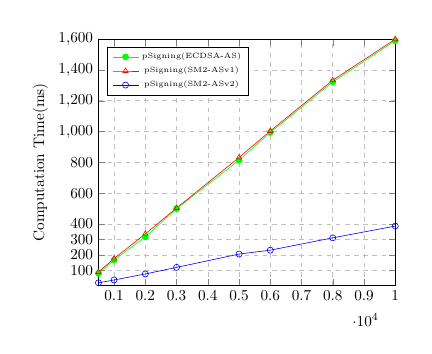
\begin{tikzpicture}[scale=0.55]
\begin{axis}[
    %xlabel={cycle index},
    ylabel={Computation Time(ms)},
    xmin=500, xmax=10000,
    ymin=0, ymax=1600,
    xtick={1000,2000,3000,4000,5000,6000,7000,8000,9000,10000},
    ytick={100,200,300,400,600,800,1000,1200,1400,1600},
    legend pos=north west,
    ymajorgrids=true,
    grid style=dashed,
    xmajorgrids=true,
    grid style=dashed,
]
\addplot[
    color=green,
    mark=*,
    ]
    coordinates {(500,80.43)(1000,166.54)(2000,316.68)(3000,499.99)(5000,813.99)(6000,994.28)(8000,1322.32)(10000,1589.63)
    };


\addplot[
    color=red,
    mark=triangle,
    ]
    coordinates {(500,89.11)(1000,176.27)(2000,336.17)(3000,504.13)(5000,832.15)(6000,1003.95)(8000,1333.51)(10000,1599.4)
    };

\addplot[
    color=blue,
    mark=o,
    ]
    coordinates {(500,18.84)(1000,37.14)(2000,76.24)(3000,118.83)(5000,205.34)(6000,230.55)(8000,310.69)(10000,387.00)
    };

    \legend{{\tiny pSigning(ECDSA-AS)},{\tiny pSigning(SM2-ASv1)},{\tiny pSigning(SM2-ASv2)}}
\end{axis}
\end{tikzpicture}
\end{minipage}
\hspace{0.01\textwidth}
\begin{minipage}[c]{0.45\textwidth}
\centering
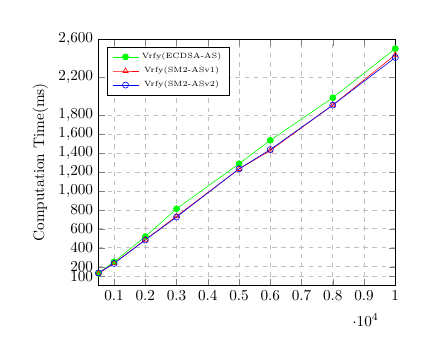
\begin{tikzpicture}[scale=0.55]
\begin{axis}[
    %xlabel={cycle index},
    ylabel={Computation Time(ms)},
    xmin=500, xmax=10000,
    ymin=0, ymax=2600,
    xtick={1000,2000,3000,4000,5000,6000,7000,8000,9000,10000},
    ytick={100,200,400,600,800,1000,1200,1400,1600,1800,2200,2600},
    legend pos=north west,
    ymajorgrids=true,
    grid style=dashed,
    xmajorgrids=true,
    grid style=dashed,
]
\addplot[
    color=green,
    mark=*,
    ]
    coordinates {(500,130.85)(1000,252.86)(2000,517.81)(3000,811.38)(5000,1285.96)(6000,1533.15)(8000,1981.72)(10000,2499.86)
    };


\addplot[
    color=red,
    mark=triangle,
    ]
    coordinates {(500,127.03)(1000,238.46)(2000,485.32)(3000,733.33)(5000,1230.41)(6000,1426.1)(8000,1904.61)(10000,2434.72)
    };

\addplot[
    color=blue,
    mark=o,
    ]
    coordinates {(500,135.11)(1000,234.80)(2000,482.16)(3000,723.98)(5000,1232.33)(6000,1435.69)(8000,1904.37)(10000,2405.78)
    };

    \legend{{\tiny Vrfy(ECDSA-AS)},{\tiny Vrfy(SM2-ASv1)},{\tiny Vrfy(SM2-ASv2)}}
\end{axis}
\end{tikzpicture}
\end{minipage}
\centering
\caption{(a) 预签名算法和 (b) 验证算法效率对比}{Efficiency comparison of (a) pre-signing and (b) verification algorithm}
\label{Efficiency comparison of (a) pre-signing and (b) verification algorithm}
\end{figure}




\section{应用} 

在本节中, 我们根据现有适配器签名应用~\cite{Poelstra2017,MalavoltaMSKM19,EsginEE20,AumayrEEFHMMR20},介绍SM2适配器签名的两个典型区块链应用: 原子交换协议和支付通道网络. 

\subsection{原子交换协议}

原子交换协议 (atomic swap) 能在无可信第三方的情况下公平地实现不同密码货币之间的交换. 用户$U_1$和$U_2$想要公平地交换不同的密码货币$c_1$和$c_2$, 其中公平性体现在双方完成交换或者双方都交换失败. 最初, 原子交换协议~\cite{Nolan2013}基于哈希函数和时间锁(timelock)设计, 可实现拥有哈希函数原像才能提取货币的功能, 时间锁保证后提取货币的用户有足够的时间进行货币提取, 但该方法要求密码货币的两种脚本语言都支持哈希原像条件脚本(preimage conditioned scripts). 随后, Poelstra~\cite{Poelstra2017}将哈希条件嵌入到签名算法中, 给出了该协议的无脚本版本. 因此, 基于适配器签名设计原子交换协议框架~\cite{Nolan2013,Poelstra2017,EsginEE20}, 在现有基于SM2签名算法的区块链应用中, 可使用SM2的适配器签名构造原子交换协议, 具体如图~\ref{Atomic swap protocol based on SM2-based adaptor signature}所示: 

\begin{itemize}

\item 协议建立阶段: $U_1$运行$\mathsf{GenR}(1^\lambda)\rightarrow (Y,y)$生成困难关系$(Y,y)$, 计算零知识证明$\mathsf{P}(Y,y)\rightarrow \pi$, 令$I=(Y,\pi)$. 生成关于传输货币$c_1$给$U_2$的预交易$tx_1$, 并生成预签名$\hat{\sigma_1}\leftarrow \mathsf{pSign}((X_1,x_1), tx_1, I)$; 将$I, \hat{\sigma_1}, tx_1$发送给$U_2$; $U_2$可验证困难实例$I$和预签名值$\hat{\sigma_1}$, 如果$\mathsf{V}(I)\rightarrow 0$或者$\mathsf{pVrfy}$$(X_1$, $tx_1$, $I$, $\hat{\sigma_1})$$\rightarrow 0$, 拒绝交易;  否则生成关于传输货币$c_2$给$U_1$的预交易$tx_2$, 并生成预签名$\hat{\sigma_2}$$\leftarrow$$\mathsf{pSign}$$((X_2$, $x_2)$, $tx_2$, $I)$; 将$\hat{\sigma_2},tx_2$发送给$U_1$;

\item 交换阶段: $U_1$验证预签名值, 如果 $\mathsf{pVrfy}(X_2$, $tx_2$, $I$, $\hat{\sigma_2})$$\rightarrow 0$, 则拒绝交易; 否则根据证据$y$, 运行适配算法$\sigma_2\leftarrow \mathsf{Adapt}(\hat{\sigma_2},y)$将$U_2$的预签名适配成SM2签名, 即获得$U_2$传输货币$c_2$给$U_1$的SM2签名值$\sigma_2$, 在链上公布$\sigma_2$可获得$c_2$; $U_2$获得签名值$\sigma_2$, 运行提取算法获得证据$y\leftarrow \mathsf{Ext}(\sigma_2,\hat{\sigma_2}, I)$, 并运行适配算法$\sigma_1\leftarrow \mathsf{Adapt}(\hat{\sigma_1},y)$, 获得$U_1$传输货币$c_1$给$U_2$的SM2签名值$\sigma_1$, 在链上公布$\sigma_1$获得$c_1$.
\end{itemize}


\begin{figure*}[!h]
\begin{center}
\fbox{\resizebox{\textwidth}{!}{ 
\begin{tabular}{ccccc}
$U_1((X_1,x_1),X_2,c_1)$ & & &     & $U_2((X_2,x_2),X_1,c_2)$\\
\hline
$\mathsf{GenR}(1^\lambda)\rightarrow (Y,y)$, $\mathsf{P}(Y,y)\rightarrow \pi$ & & &  &  \\
$I=(Y,\pi)$, $\hat{\sigma_1}\leftarrow \mathsf{pSign}((X_1,x_1), I, tx_1)$& & $\xrightarrow{I, \hat{\sigma_1}, tx_1}$ &  & If $\mathsf{V}(I)\rightarrow 0$ or $\mathsf{pVrfy}(X_1, tx_1, I, \hat{\sigma_1})\rightarrow 0$ \\
& &  &  & Output $\bot$\\
If $\mathsf{pVrfy}(X_2, tx_2, I, \hat{\sigma_2})\rightarrow 0$ & & $\xleftarrow{\hat{\sigma_2}, tx_2}$ &  & else, $\hat{\sigma_2}\leftarrow \mathsf{pSign}((X_2,x_2), tx_2, I)$ \\
Output $\bot$& &  &  & \\
eLse, $\sigma_2\leftarrow \mathsf{Adapt}(\hat{\sigma_2},y)$& & &  & \\
Publish $\sigma_2$ on blockchain& & $\xrightarrow{\sigma_2}$&  & $y'\leftarrow \mathsf{Ext}(\sigma_2, \hat{\sigma_2}, I)$ \\
& & &  & $\sigma_1\leftarrow \mathsf{Adapt}(\hat{\sigma_1},y)$\\
& & &  & Publish $\sigma_1$ on blockchain\\
\end{tabular}}}
\caption{基于SM2适配器签名构造原子交换协议}{Atomic swap protocol based on SM2-based adaptor signature}
\label{Atomic swap protocol based on SM2-based adaptor signature}
\end{center}
\end{figure*}

\subsection{支付通道网络}
支付通道网络(payment channel network, PCN)~\cite{DeckerW15,PD2016,PC2018,MalavoltaMSKM19,AumayrEEFHMMR20}是目前解决区块链可扩展性差, 吞吐量低的主流方案. 具体地说, 区块链上每笔交易需要各方(矿工)认可和存储, 导致交易吞吐量较差, 但PCN可通过将部分交易移到链下来提高吞吐量. 在PCN中, 交易双方可将货币锁定在一个通道中, 只要有足够的余额, 就可以进行即时和任意多次的交易. 目前, 最受欢迎的PCN应用是基于比特币的闪电网络~\cite{PD2016}. PCN允许各方进行多跳支付, 即没有直接通道的参与方可以使用中介节点的通道来实现支付. 在多跳支付中, 各方需要同步路线上每个通道信息, 要求所有通道都同步更新, 或者都不更新. 闪电网络通过使用哈希锁合约(hash-time lock contract, HTLC)实现上述要求. 然而, Malavolta等~\cite{MalavoltaMSKM19}提出虫洞攻击可破坏HTLC机制的安全性, 并基于ECDSA适配器签名构造匿名多跳锁(anonymous multi-hop lock, AMHL)构建了安全的PCN.

在现有基于SM2签名算法的区块链应用中, 我们可使用SM2的适配器签名, 采用Malavolta等~\cite{MalavoltaMSKM19,EsginEE20}的构造框架, 实现PCN的多跳支付. 具体应用中, 发送者$S$(或$U_0$)通过中介节点$U_1,\cdots,U_{k−1}$向接收方$R$(或$U_k$)进行支付, 为了方便, 我们省略中介节点的费用, 令$(X_j, x_j)$是$U_j$的SM2签名公私钥对, $G$是阶为$n$的基点, $tx_j$是指$U_j$到$U_{j+1}$交易. 具体协议如图~\ref{Multi-hop payments based on SM2-based adaptor signature}: 

\begin{itemize}
\item 建立阶段: $S$选择随机数$l_j\in \mathbb{Z}_n$, $j=0,\cdots,k-1$, 计算$y_j=\sum_{i=0}^{j}l_i \bmod n$和$Y_j= y_jG$, 并证明$\pi_{Y_j}\leftarrow \mathsf{P}(Y_j,y_j)$, 计算$Z_j=y_jX_j+Y_j$, $I_j=(G,(Y_j,\pi_{Y_j}),X_j,Z_j)$, $\pi_j\leftarrow \mathsf{P}(I_j)$, $j=0,\cdots,k-1$. $S$发送$(Y_{j−1},Y_j,Z_j,\pi_j,l_j)$给$U_j$, 发送$(Y_{k−1},y_{k-1})$给$R$. $U_j$可验证传输值的正确性, $\mathsf{V}(I_j)\rightarrow 1$和 $Y_j-Y_{j−1}=l_jG$, 否则拒绝交易. $R$ 可验证$Y_{k−1}=y_{k-1}G$, 否则拒绝交易. 

\item 支付阶段: $S$计算预签名$\hat{\sigma}_0$ $\leftarrow$ $\mathsf{pSign}$ $((X_0$, $x_0)$, $tx_0$, $I_0)$并发送给$U_1$, $U_1$验证预签名值$\mathsf{pVrfy}$$(X_0$, $tx_0$, $I_0$, $\hat{\sigma}_0)\rightarrow 1$, 否则拒绝交易. $U_j$从$U_{j−1}$收到预签名$\hat{\sigma}_{j−1}$, 并验证正确后, 计算预签名$\hat{\sigma}_j\leftarrow\mathsf{pSign}((X_j, x_j),tx_j,I_j)$, $j = 1,\cdots,k−1$发送给$U_{j+1}$. 所有预签名传输完成, 即$R$获得预签名$\hat{\sigma}_{k−1}$, $U_j$获得预签名$\hat{\sigma}_{j−1}$, 并计算了预签名值$\hat{\sigma}_{j}$. $R$根据证据$y_{k−1}$可将预签名值$\hat{\sigma}_{k-1}$适配成SM2签名值$\sigma_{k−1}\leftarrow \mathsf{Adapt}(\hat{\sigma}_{k-1},y_{k-1})$获得$U_{k−1}$的支付. $R$发送$\sigma_{k−1}$给$U_{k−1}$; $U_{k−1}$可验证$\sigma_{k−1}$的正确性, $\mathsf{Vrfy}$$(X_{k-1}$, $tx_{k-1}$, $\sigma_{k-1})$$\rightarrow 1$, 否则拒绝交易, 并运行提取算法提取证据$y_{k-1}$$\leftarrow$ $\mathsf{Ext}($$\sigma_{k-1}$, $\hat{\sigma}_{k-1}$, $I_{k-1})$, 计算$y_{k-2} = y_{k-1}−l_{k−1}$, 运行适配算法计算SM2签名值$\sigma_{k−2}\leftarrow \mathsf{Adapt}(\hat{\sigma}_{k-2}, y_{k-2})$获得$U_{k−2}$的支付, 并将$\sigma_{k−2}$发送给$U_{k−2}$. 如此, $U_j$获得SM2签名$\sigma_j$可通过提取算法获得$y_j\leftarrow \mathsf{Ext}(\sigma_j,\hat{\sigma}_j,I_j)$, 并计算出$y_{j-1}=y_j-l_{j}$, 然后通过适配算法计算SM2签名$\sigma_{j-1}\leftarrow \mathsf{Adapt}(\hat{\sigma}_{j-1},y_{j-1})$获得$U_{j-1}$的支付, 并将$\sigma_{j-1}$发送给$U_{j-1}$, $j=k-1,k-2,\cdots,1$. 最后, $U_{1}$可计算SM2签名$\sigma_0$获得$S$的支付. 
\end{itemize}

\begin{figure*}[!h]
\begin{center}
\fbox{\resizebox{\textwidth}{!}{ 
\begin{tabular}{ccccc}
$S(x_0,X_j),j = 0,1,\cdots,k−1$ & & Setup &     & $U_{j}(x_j,X_j),j = 1,\cdots,k$\\
\hline
$l_j\leftarrow_r \mathbb{Z}_n$, $j=0,\cdots,k-1$& & & &  \\
$y_j=\sum_{i=0}^{j}l_i \bmod n$& & &  & \\
$Y_j= y_jG$, $\pi_{Y_j}\leftarrow \mathsf{P}(Y_j,y_j)$ & & &  & \\ 
$Z_j=y_jX_j+Y_j$ & & &  & \\
$I_j=(G,(Y_j,\pi_{Y_j}),X_j,Z_j)$&  & $\xrightarrow{Y_{j−1},Y_j,Z_j,\pi_j,l_j}U_{j}$ &  & If $\mathsf{V}(I_j)\rightarrow 0$ or $Y_j-Y_{j−1}\not=l_jG$, $U_{j}$ aborts.\\
$\pi_j\leftarrow \mathsf{P}(I_j)$, $j=0,\cdots,k-1$& &$\xrightarrow{Y_{k−1},y_{k-1}}R$ &  & If $Y_{k−1}\not=y_{k-1}G$, $R$ aborts. \\
\hline
 & & Payment &  &  \\
\hline
$S\xrightarrow{\hat{\sigma}_0\leftarrow \mathsf{pSign}((X_0, x_0), tx_0, I_0)}U_1\xrightarrow{\cdots}$&$\cdots$&$\xrightarrow{\hat{\sigma}_{j-1}}U_{j}\xrightarrow{\hat{\sigma}_{j}\leftarrow \mathsf{pSign}((X_j, x_j), tx_j, I_j)}U_{j+1}\xrightarrow{\hat{\sigma}_{j+1}}$& $\cdots$ & $\xrightarrow{\cdots}U_{k-1}\xrightarrow{\hat{\sigma}_{k-1}\leftarrow \mathsf{pSign}((X_{k-1}, x_{k-1}), tx_{k-1}, I_{k-1})}R$ \\
$S\xleftarrow{\sigma_0\leftarrow \mathsf{Adapt}(\hat{\sigma}_0,y_0)}U_1\xleftarrow{\cdots}$&$\cdots$&$\xleftarrow{\sigma_{j-1}}U_{j}\xleftarrow{\sigma_{j}\leftarrow \mathsf{Adapt}(\hat{\sigma}_{j},y_{j})}U_{j+1}\xleftarrow{\sigma_{j+1}}$& $\cdots$ & $\xleftarrow{\cdots}U_{k-1}\xleftarrow{\sigma_{k−1}\leftarrow \mathsf{Adapt}(\hat{\sigma}_{k-1},y_{k-1})}R$ \\
\end{tabular}}}
\caption{基于SM2适配器签名的多跳支付协议}{Multi-hop payments based on SM2-based adaptor signature}
\label{Multi-hop payments based on SM2-based adaptor signature}
\end{center}
\end{figure*}

\section{总结}
针对现有区块链技术的可扩展性差、交易吞吐量低等问题, 同时秉承积极推广国密算法应用的理念, 填补现有SM2适配器签名的空白, 我们基于``自证明结构''设计可证明安全的SM2适配器签名方案, 并且根据SM2签名的结构, 采用``离线证明技术'', 在不影响可证明安全性的情况下, 构造更加高效的SM2适配器签名方案. 该方案与现有ECDSA适配器签名方案相比, 在线预签名过程不需要额外的零知识证明, 计算效率更高, 应用优势更广. 最后, 我们基于适配器签名的现有应用, 分别给出SM2适配器签名在区块链上的两个具体应用, 为后续SM2签名算法的应用推广提供参考. 


\begin{thebibliography}{10}
\providecommand{\url}[1]{\texttt{#1}}
\providecommand{\urlprefix}{URL }

\bibitem{Nak08}
Nakamoto, S.: Bitcoin: A peer-to-peer electronic cash system (2008),
  \url{https://nakamotoinstitute.org/bitcoin/}

\bibitem{BanoSAAMMD19}
Bano, S., Sonnino, A., Al{-}Bassam, M., Azouvi, S., McCorry, P., Meiklejohn,
  S., Danezis, G.: Sok: Consensus in the age of blockchains. In: Proceedings of
  the 1st {ACM} Conference on Advances in Financial Technologies, {AFT} 2019,
  Zurich, Switzerland, October 21-23, 2019. pp. 183--198. {ACM} (2019),
  \url{https://doi.org/10.1145/3318041.3355458}

\bibitem{GudgeonMRMG19}
Gudgeon, L., Moreno{-}Sanchez, P., Roos, S., McCorry, P., Gervais, A.: Sok: Off
  the chain transactions. {IACR} Cryptol. ePrint Arch.  2019,  360 (2019),
  \url{https://eprint.iacr.org/2019/360}

\bibitem{ZamyatinAZKMKK19}
Zamyatin, A., Al{-}Bassam, M., Zindros, D., Kokoris{-}Kogias, E.,
  Moreno{-}Sanchez, P., Kiayias, A., Knottenbelt, W.J.: Sok: Communication
  across distributed ledgers. {IACR} Cryptol. ePrint Arch.  2019,  1128 (2019),
  \url{https://eprint.iacr.org/2019/1128}

\bibitem{AumayrEEFHMMR20}
Aumayr, L., Ersoy, O., Erwig, A., Faust, S., Host{\'{a}}kov{\'{a}}, K., Maffei,
  M., Moreno{-}Sanchez, P., Riahi, S.: Generalized bitcoin-compatible channels.
  {IACR} Cryptol. ePrint Arch.  2020,  476 (2020),
  \url{https://eprint.iacr.org/2020/476}

\bibitem{SG2018}
Shan J Y, Gao S. Research progress on theory of blockchains[J]. Journal of Cryptologic Research, 2018, 5(5).\\
单进勇, 高胜. 区块链理论研究进展[J]. 密码学报, 2018, 5(5).

\bibitem{PC2018}
Bitcoin Wiki: Payment channels  (2018), \url{https : / / en . bitcoin . it /
  wiki/Payment channels}

\bibitem{PD2016}
J. Poon and T. Dryja: The bitcoin lightning network: Scalable off-chain
  instant payments  (2016), \url{https://lightning.network/lightning-
  network-paper.pdf}

\bibitem{raidEX}
Update from the Raiden team on development progress, announcement of raidEX. \url{https://tinyurl.com/z2snp9e. Feb. 2017.}

\bibitem{Poelstra2016}
A. Poelstra. Lightning in Scriptless Scripts. mimblewimble team mailing list. \url{https : / / lists . launchpad . net/mimblewimble/msg00086.html.}

\bibitem{DeckerW15}
Decker, C., Wattenhofer, R.: A fast and scalable payment network with bitcoin
  duplex micropayment channels. In: Pelc, A., Schwarzmann, A.A. (eds.)
  Stabilization, Safety, and Security of Distributed Systems - 17th
  International Symposium, {SSS} 2015, Edmonton, AB, Canada, August 18-21,
  2015, Proceedings. Lecture Notes in Computer Science, vol. 9212, pp. 3--18.
  Springer (2015), \url{https://doi.org/10.1007/978-3-319-21741-3\_1}

\bibitem{EckeyFHR20}
Eckey, L., Faust, S., Host{\'{a}}kov{\'{a}}, K., Roos, S.: Splitting payments
  locally while routing interdimensionally. {IACR} Cryptol. ePrint Arch.  2020,
   555 (2020), \url{https://eprint.iacr.org/2020/555}

\bibitem{MalavoltaMSKM19}
Malavolta, G., Moreno{-}Sanchez, P., Schneidewind, C., Kate, A., Maffei, M.:
  Anonymous multi-hop locks for blockchain scalability and interoperability.
  In {NDSS} 2019,
  \url{https://www.ndss-symposium.org/ndss-paper/anonymous-multi-hop-locks-for-blockchain-scalability-and-interoperability/}

\bibitem{MillerBBKM19}
Miller, A., Bentov, I., Bakshi, S., Kumaresan, R., McCorry, P.: Sprites and
  state channels: Payment networks that go faster than lightning. In: Goldberg,
  I., Moore, T. (eds.) Financial Cryptography and Data Security - 23rd
  International Conference, {FC} 2019. Lecture Notes in Computer
  Science, vol. 11598, pp. 508--526. Springer (2019),
  \url{https://doi.org/10.1007/978-3-030-32101-7\_30}

\bibitem{Nolan2013}
Nolan, T.: Alt chains and atomic transfers, \url{https://bitcointalk.org/index.php? topic=193281.msg2224949#msg2224949}

\bibitem{Poelstra2017}
Poelstra, A.: Adaptor signatures and atomic swaps from scriptless scripts,
\url{https://github.com/ElementsProject/scriptless-scripts/tree/master/slides/2017-05-milan-meetup}

\bibitem{DeshpandeH20}
Deshpande, A., Herlihy, M.: Privacy-preserving cross-chain atomic swaps. In:
  Bernhard, M., Bracciali, A., Camp, L.J., Matsuo, S., Maurushat, A., R{\o}nne,
  P.B., Sala, M. (eds.) Financial Cryptography and Data Security - {FC} 2020,
  \url{https://doi.org/10.1007/978-3-030-54455-3\_38}

\bibitem{Gugger20}
Gugger, J.: Bitcoin-monero cross-chain atomic swap. {IACR} Cryptol. ePrint
  Arch.  2020,  1126 (2020), \url{https://eprint.iacr.org/2020/1126}

\bibitem{SM2} GM/T 0003-2012,Public Key Cryptographic Algorithm SM2 Based on Elliptic Curves. 2010 
  \url{http://www.gmbz.org.cn/main/viewfile/2018 0108015515787986.html} \\
  GM/T 0003-2012, SM2 椭圆曲线公钥密码算法.2010.

\bibitem{SM2-survey} Wang Z H,Zhang Z F. Overview on Public Key Cryptographic Algorithm SM2 Based on Elliptic Curves. Journal of Information Security Research, 2016(11).\\
汪朝晖, 张振峰. SM2椭圆曲线公钥密码算法综述[J]. 信息安全研究, 2016(11).

\bibitem{Sch89}
Schnorr, C.: Efficient identification and signatures for smart cards. In:
  Advances in Cryptology - {CRYPTO} '89, 9th Annual International Cryptology
  Conference, Santa Barbara, California, USA, August 20-24, 1989, Proceedings.
  pp. 239--252 (1989), \url{https://doi.org/10.1007/0-387-34805-0\_22}

\bibitem{ErwigFHMR2021}
Erwig, A., Faust, S., Host{\'{a}}kov{\'{a}}, K., Maitra, M. Riahi, S.: Two-Party Adaptor Signatures From Identification Schemes. Public-Key Cryptography, 2021.

\bibitem{ECDSA}
{American National Standards Institute}: X9.62: Public key cryptography for the
  financial services industry: The elliptic curve digital signature algorithm
  (ecdsa) (2005)

\bibitem{rfc6605}
Hoffman, P.E., Wijngaards, W.C.A.: Elliptic curve digital signature algorithm
  {(DSA)} for {DNSSEC}. {RFC}  6605,  1--8 (2012),
  \url{https://doi.org/10.17487/RFC6605}

\bibitem{DucasLLSSS2018}
Ducas, L., Lepoint, T., Lyubashevsky, V., Schwabe, P., Seiler, G., Stehlé, D.: Crystals–Dilithium: Digital signatures from module lattices. In: CHES. vol. 2018-1
(2018)

\bibitem{EsginEE20}
Esgin, M.F., Ersoy, O., Erkin, Z.: Post-quantum adaptor signatures and payment
  channel networks. In: Chen, L., Li, N., Liang, K., Schneider, S.A. (eds.)
  Computer Security - {ESORICS} 2020, Lecture Notes in Computer Science, vol. 12309, pp.
  378--397. Springer (2020),
  \url{https://doi.org/10.1007/978-3-030-59013-0\_19}

\bibitem{PA18}
Moreno{-}Sanchez, P., Kate, A.. Scriptless Scripts with ECDSA. lightning-dev mailing list. \url{https://lists.linuxfoundation.org/pipermail/lightning-dev/attachments/20180426/fe978423/attachment-0001.pdf}

\bibitem{Fischlin05}
Fischlin, M.: Communication-efficient non-interactive proofs of knowledge with
  online extractors. In: Shoup, V. (ed.) Advances in Cryptology - {CRYPTO}
  2005: 25th Annual International Cryptology Conference, Santa Barbara,
  California, USA, August 14-18, 2005, Proceedings. Lecture Notes in Computer
  Science, vol. 3621, pp. 152--168. Springer (2005),
  \url{https://doi.org/10.1007/11535218\_10}

\bibitem{ZhangYZC15}
Zhang, Z., Yang, K., Zhang, J., Chen, C.: Security of the {SM2} signature
  scheme against generalized key substitution attacks. In: Chen, L., Matsuo, S.
  (eds.) Security Standardisation Research - Second International Conference,
  {SSR} 2015, Tokyo, Japan, December 15-16, 2015, Proceedings. Lecture Notes in
  Computer Science, vol. 9497, pp. 140--153. Springer (2015),
  \url{https://doi.org/10.1007/978-3-319-27152-1\_7}



\end{thebibliography}


\end{document}
